\chapter{Experimental Results}
  \noindent This chapter is devoted to the experimental evaluation of WFQI on classic RL problems.
  We test the proposed algorithm on two versions of the puddle world and on the activity swing-up. Both
  environments have a continuous state-space and discrete action-space. We evaluate the performance of WFQI in terms
  of expected return under different numbers of source/target samples varying also the number of source tasks involved.\newline
  We start presenting the metrics we adopt to evaluate our approach and finally, we report the results over
  the different environments.

  \section{Evaluation Metrics}
    \noindent Defining a metric for the notion the notion of "good transfer" is, in general, a hard task and
    in literature different metrics have been proposed. As already highlighted in the previous section
    we plot the results in terms of expected discounted return $J_{\pi}$ of the best policy learnt by WFQI
    after performing the transfer:
    \begin{equation}
      J_{\pi} = \sum_{t=0}^{T} \gamma^{t}R(s_{t}, \pi(s_{t}))
    \end{equation}
    The resulting graphs are quite useful because they permit to have a graphical overview
    of the jumpstart improvement and of the time to learn the optimal policy from the source
    and target samples.\newline

  \section{The Puddle World Environment}
    \noindent In this set of experiments we deal with MDPs with continuous state space (and discrete action space).\newline
    Puddle-world is an environment similar to grid-world where the agent must move toward a safe area while avoiding
    to walk inside the puddles. Only four actions (N,S,W,E) are allowed in each state. When the agent bump in the
    border of the environment it always return to the state where the action was initially performed.\newline
    The settings for the experiment is the following: two task (target and source), $\gamma = 0.99$, the size is $10 \times 10$,
    and the maximum horizon is set to 30 iterations.\newline

    \noindent Puddles are modeled as (inverse) bivariate gaussian:
    \begin{equation}
      \begin{multlined}
        P(x,y) = - \frac{1}{2 \pi \sigma_x \sigma_y \sqrt{1 - \rho}} e^{-\frac{z}{2(1-\rho)^{2}}} \\
        z = \frac{(x - \mu_x )^2}{\sigma_x^2} - \frac{2 \rho (x-\mu_x)(y-\mu_y)}{\sigma_x \sigma_y} + \frac{(y - \mu_y )^2}{\sigma_y^2} \\
        \rho = \frac{\sigma_{xy}}{\sigma_x \sigma_y} \\
      \end{multlined}
    \end{equation}

    \begin{figure}[H]
      \centering
      \includegraphics[scale=0.6]{images/puddleex.eps}
      \caption{An example puddle world environment, in red the FQI policy.}
      \label{puddleex}
    \end{figure}

    \noindent We propose two variations of the puddle world environment: in the first one when the agent comes close to a puddle he
    receives a penalty proportional to the distance from the centre of the puddle; in the second variation when the agent come close
    to a puddle the length of the step reduces proportionally with respect to the distance from the center of the puddle.\newline

    \noindent In the first variation the reward for $(s,a)$ is given by the following set of equations. Let be $\mathcal{U}$ the set of puddles then:
    \begin{equation}
      r(s,a) =
      \begin{cases}
        \mathcal{N}(0,0.01) + \sum_{u \in \mathcal{U}} 100 P_{u}(s') & s' \textit{ is at goal} \\
        -1 + \mathcal{N}(0,0.01) + \sum_{u \in \mathcal{U}} 100 P_{u}(s') & s' \textit{ otherwise} \\
      \end{cases}
      \label{rw-puddle}
    \end{equation}
    The dynamics is simply given by modifying deterministically the coordinates of $s$ depending on the action $a$ chosen by
    the agent, the step-lenght $\alpha$ is unitary. Finally we add a Gaussian noise $\mathcal{N}(0,0.04)$ to both the coordinates
    to obtain $s'$.\newline

    \noindent In the second variation the reward is still given by Equation \ref{rw-puddle}, but the dynamics is now dependent also
    on the position of the agent. In particular $\alpha$ is no more unitary but given by the following equation:
    \begin{equation}
      \alpha = \frac{1}{1 + 30\sum_{u \in \mathcal{U}} P_{u}(s')}
    \end{equation}
    When the agent comes closer to the center of a puddle $\alpha \rightarrow 0$.

  \section{Target and Sources Tasks}
    \noindent In this section, we present the tasks involved in the experiments. The source tasks have different degrees
    of similarity with respect to the target task. The source task 3 (figure \ref{source3}) has the highest similarity
    but the puddles are slightly misplaced and the goal region is smaller and shifted on the right of the space. The source
    task 1 (figure \ref{source1}) maintains some similarities with the target but a large puddle on the bottom-left corner
    may produce very different policies. The last source task (figure \ref{source2}) is the one that has the highest
    differences with respect to the target, indeed the puddle configuration is very different.

    \begin{figure}[H]
      \centering
      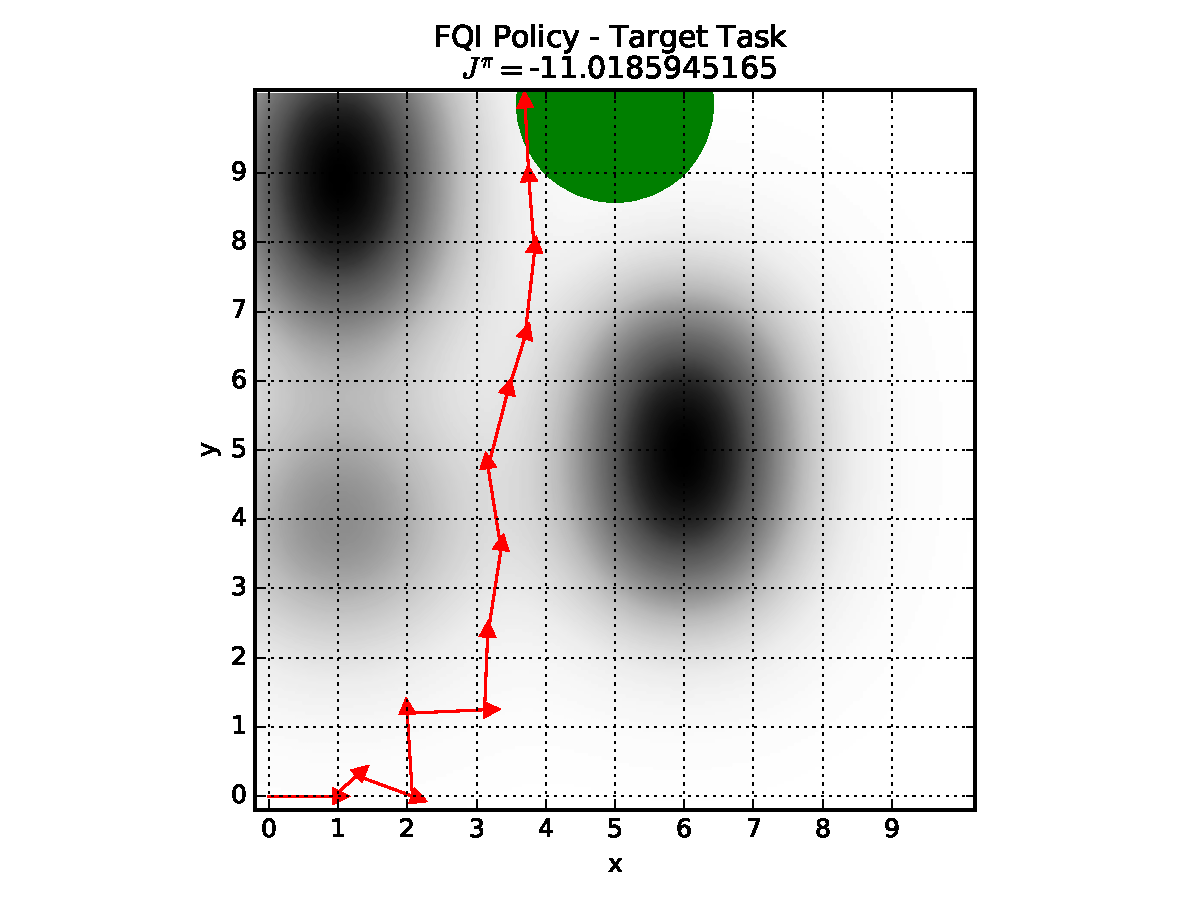
\includegraphics[scale=0.6]{images/target.pdf}
      \caption{The target task used in the experiments, in red the FQI policy.}
      \label{target}
    \end{figure}
    %
    \begin{figure}[H]
      \centering
      \includegraphics[scale=0.6]{images/source1.eps}
      \caption{Source task 1 used in the experiments, in red the FQI policy.}
      \label{source1}
    \end{figure}
    %
    \begin{figure}[H]
      \centering
      \includegraphics[scale=0.6]{images/source2.eps}
      \caption{Source task 2 used in the experiments, in red the FQI policy.}
      \label{source2}
    \end{figure}
    %
    \begin{figure}[H]
      \centering
      \includegraphics[scale=0.6]{images/source3.eps}
      \caption{Source task 3 used in the experiments, in red the FQI policy.}
      \label{source3}
    \end{figure}
    %

  \section{Results - Puddle World Version 1}
    \noindent This version of puddle world is meant to test the reward transfer capability of the algorithm. In this scenario when the
    agent comes closer to a puddle it receives a penalty on the reward proportional to the distance with respect
    to the centre of the puddle. The dynamics of the agent are unchanged (ie. the step remains unitary).\newline
    From the perspective of the weight calculation this means that only the weight associated with the reward needs to be estimated,
    the weights associated with the dynamics are always unitary.\newline
    In the following experiments, the results are averaged over 50 runs, the initial position of the agent is randomized
    at each run in the area $[0,2][0,2]$.\newline

    \noindent The parameters for the tree-based WFQI algorithm are: 50 estimators, 5 random splits and 2 minimum samples per leaf.
    Source samples are collected using the red policies reported in the previous figures.

    \subsection{Ideal Weights}
    \noindent For this set of experiments we assume to be able to calculate the ideal weights, that is we assume
    to perfectly know the model of the reward (the dynamics are identical in both the source and target task).
    Given a perfect knowledge of the model of the environment, it is possible to obtain a perfect estimation of
    the weights leading to an unbiased use of the source samples in the target task.

    \begin{figure}[H]
      \centering
      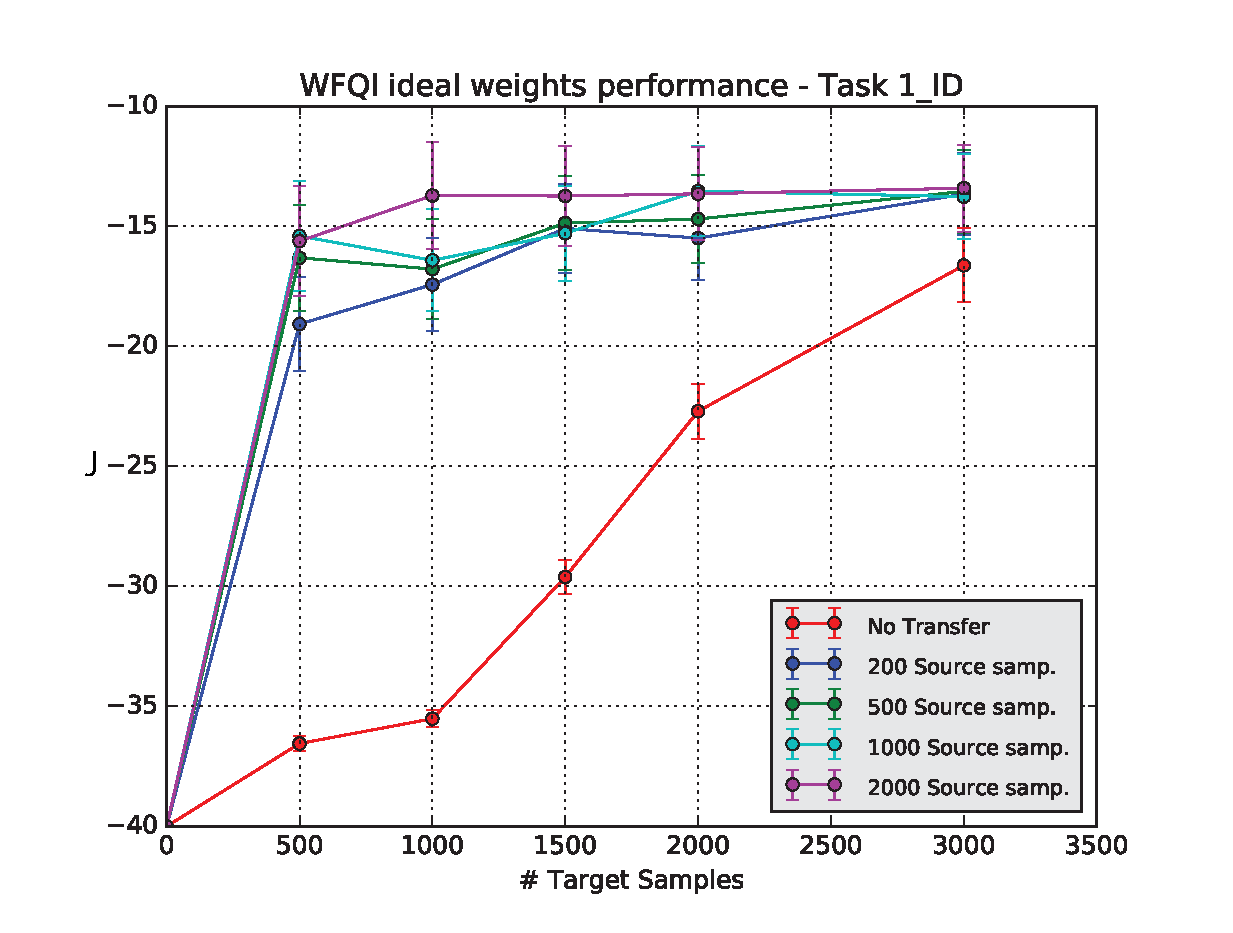
\includegraphics[scale=0.5]{images/WFQIPerf1_ID.eps}
      \caption{WFQI performance Source 1/Target task, ideal weights}
      \label{perf1ID}
    \end{figure}
    %
    \begin{figure}[H]
      \centering
      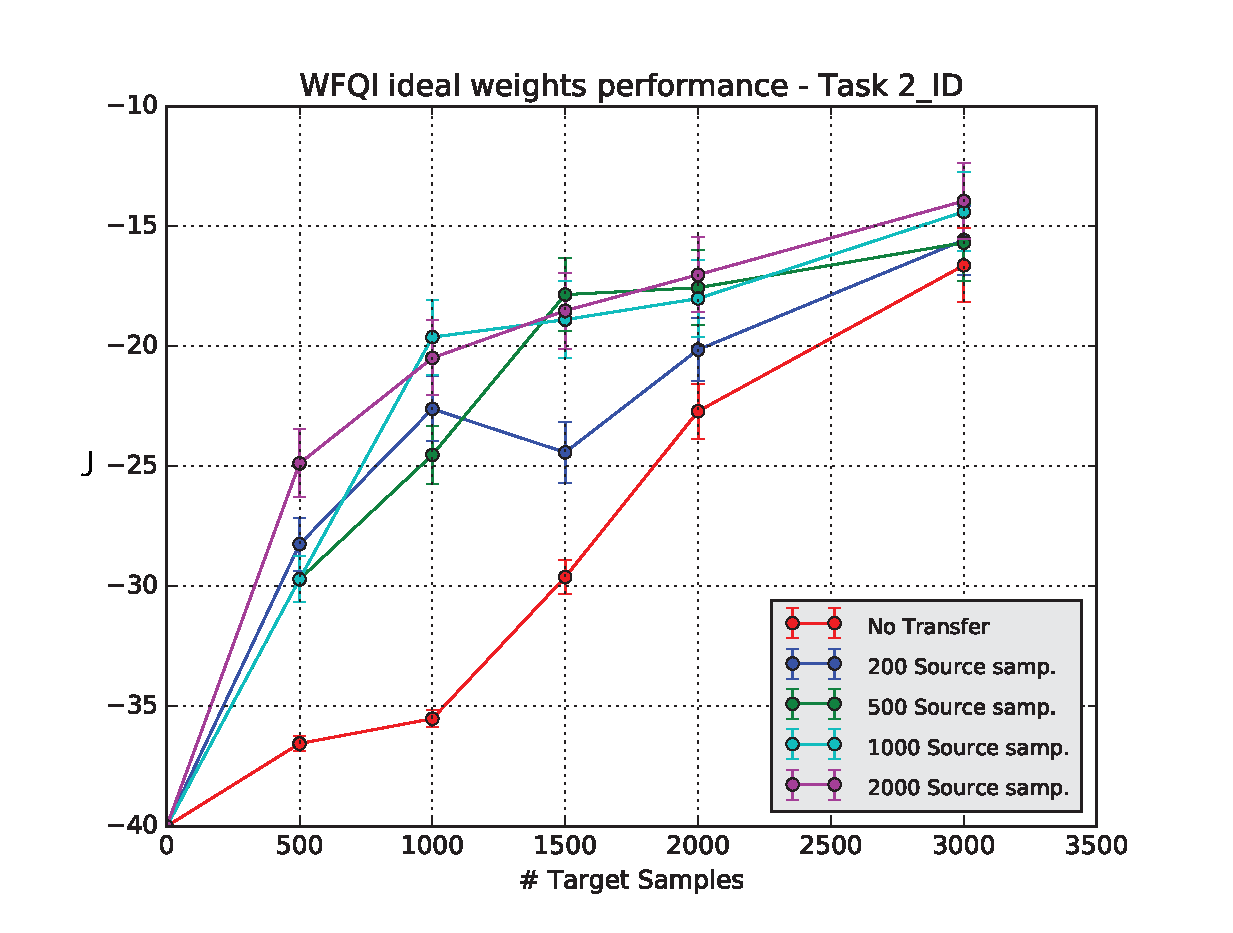
\includegraphics[scale=0.5]{images/WFQIPerf2_ID.eps}
      \caption{WFQI performance Source 2/Target task, ideal weights}
      \label{perf2ID}
    \end{figure}
    %
    \begin{figure}[H]
      \centering
      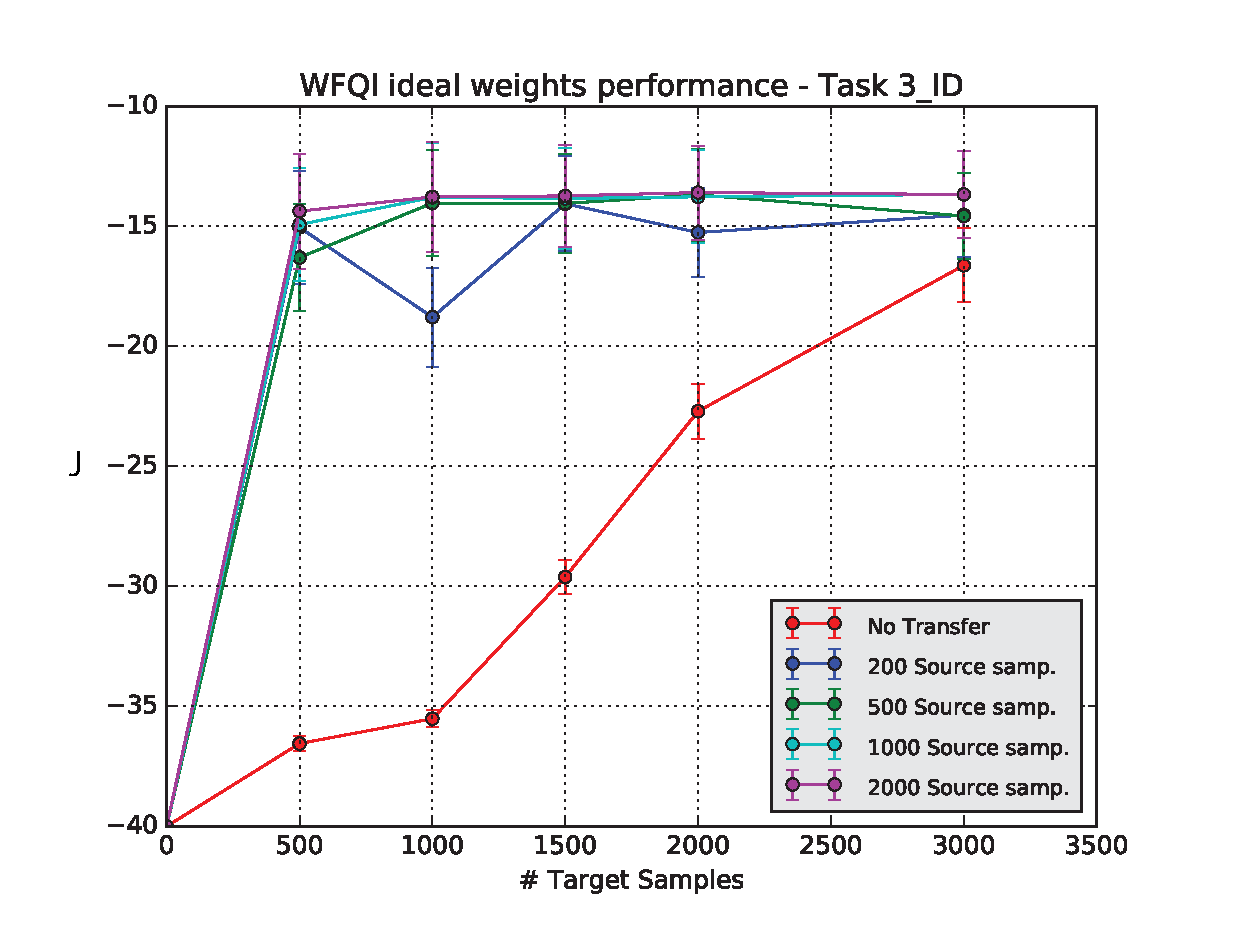
\includegraphics[scale=0.5]{images/WFQIPerf3_ID.eps}
      \caption{WFQI performance Source 3/Target task, ideal weights}
      \label{perf3ID}
    \end{figure}
    %

    \noindent In this last set of experiments the samples are transferred from all
    the source tasks toward the target in equal quantities.

    \begin{figure}[H]
      \centering
      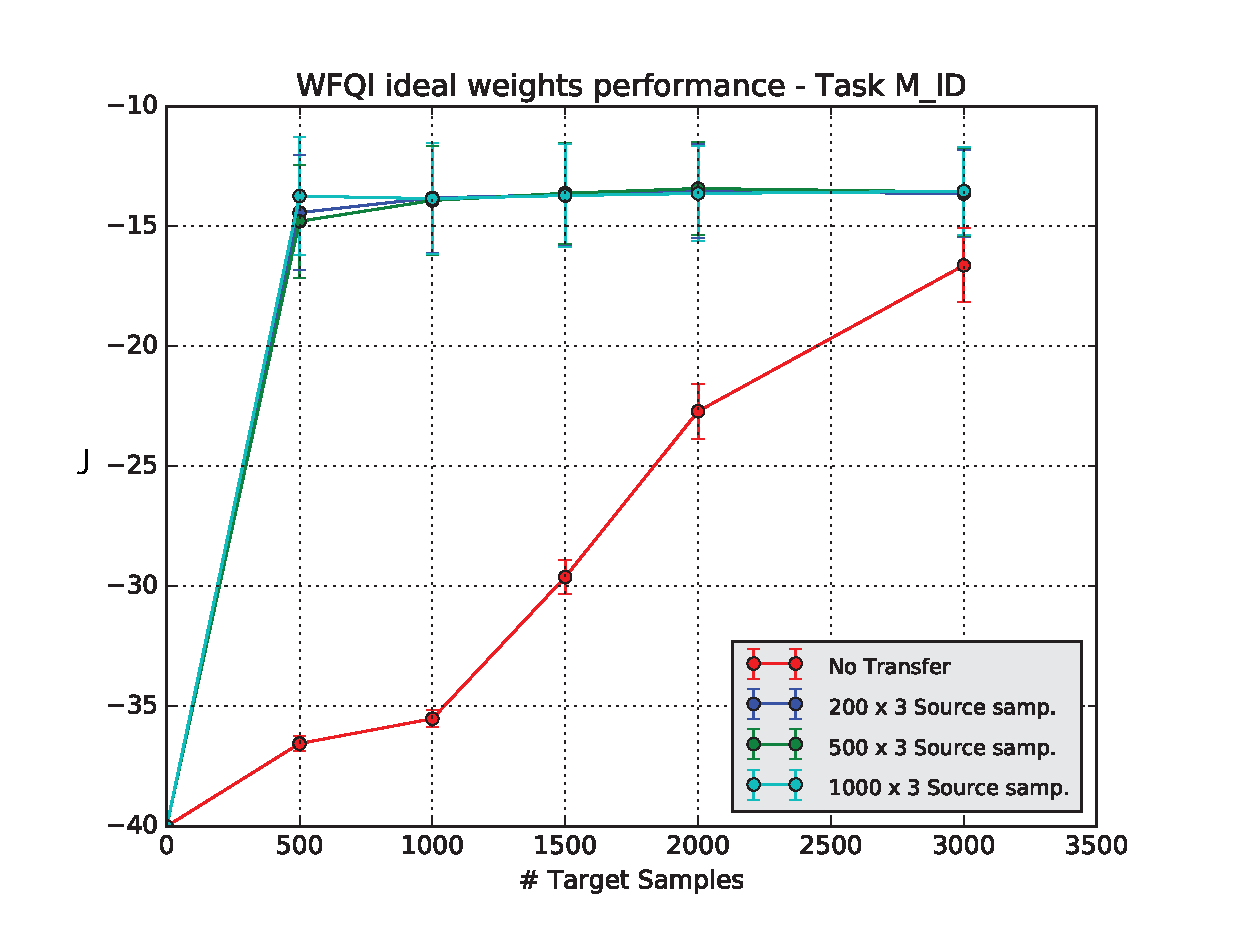
\includegraphics[scale=0.5]{images/WFQIPerfM_ID.eps}
      \caption{WFQI performance Source 1/2/3/Target task, ideal weights}
      \label{perfMID}
    \end{figure}
    %

    \noindent The results reflect the theoretical expectation: the best performances are achieved
    with the source tasks 1 and 3, on the other side, the source task 2 appear to be of little help.\newline
    Another important observation is that our algorithm is successfully able
    to limit the phenomena of the negative transfer; indeed the performance in figure \ref{perfMID}
    seems to not be influenced by the bad sample present in the source task 2.

    \subsection{Estimated Weights}
    \noindent For this set of experiments we assume to be not able to calculate the ideal weights, they are calculated
    using algorithm \ref{rw_weight_est}. These algorithms provide only an
    estimation of the real weights, therefore the use of the corresponding source samples in the target
    task is not perfectly unbiased (as in the previous scenario). A theoretical bounds over the introduced
    error has been given in the next chapter. Weights are estimated according to Equation \ref{eur}.

    \begin{figure}[H]
      \centering
      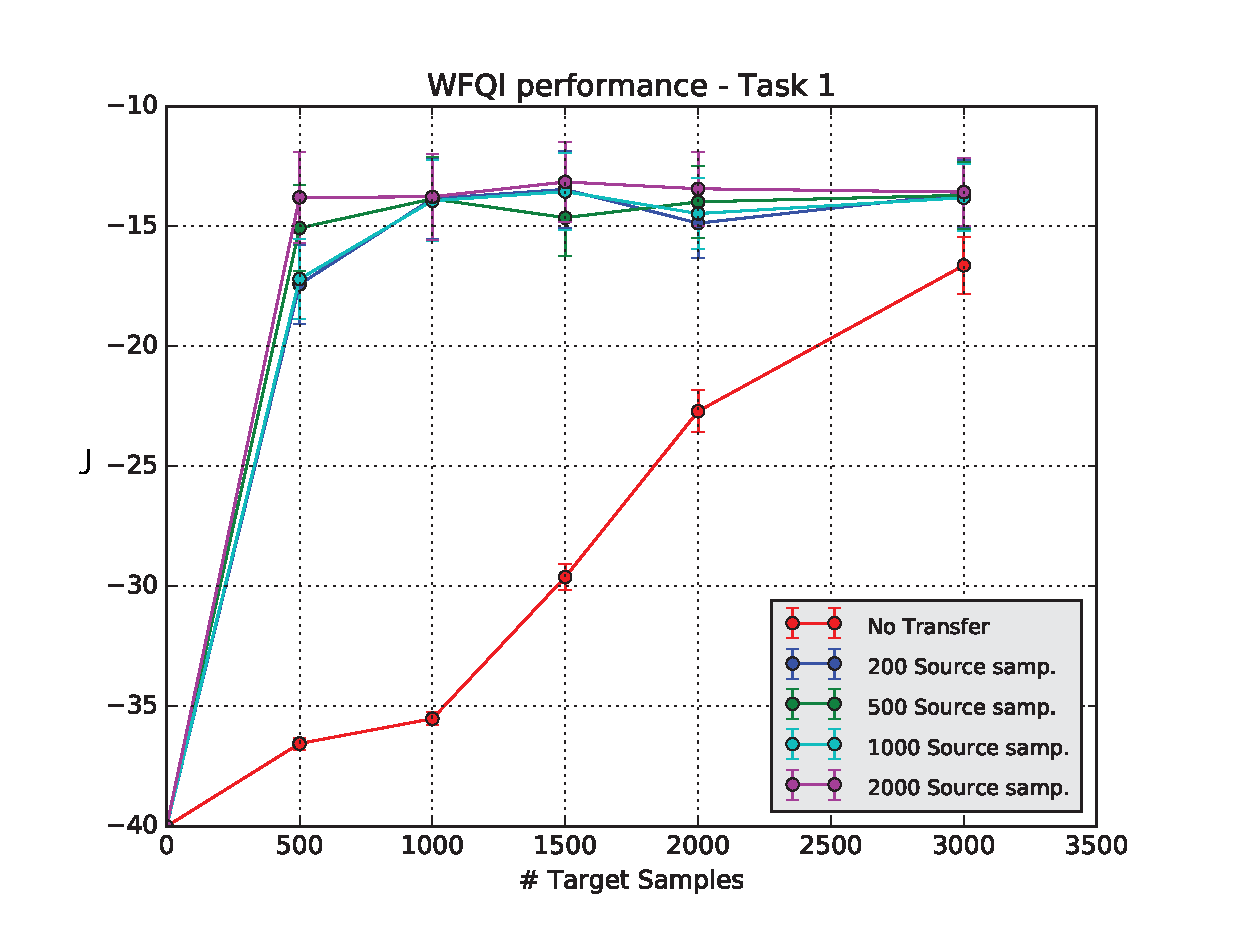
\includegraphics[scale=0.5]{images/WFQIPerf1.eps}
      \caption{WFQI performance Source 1/Target task, est. weights}
      \label{perf1E}
    \end{figure}
    %
    \begin{figure}[H]
      \centering
      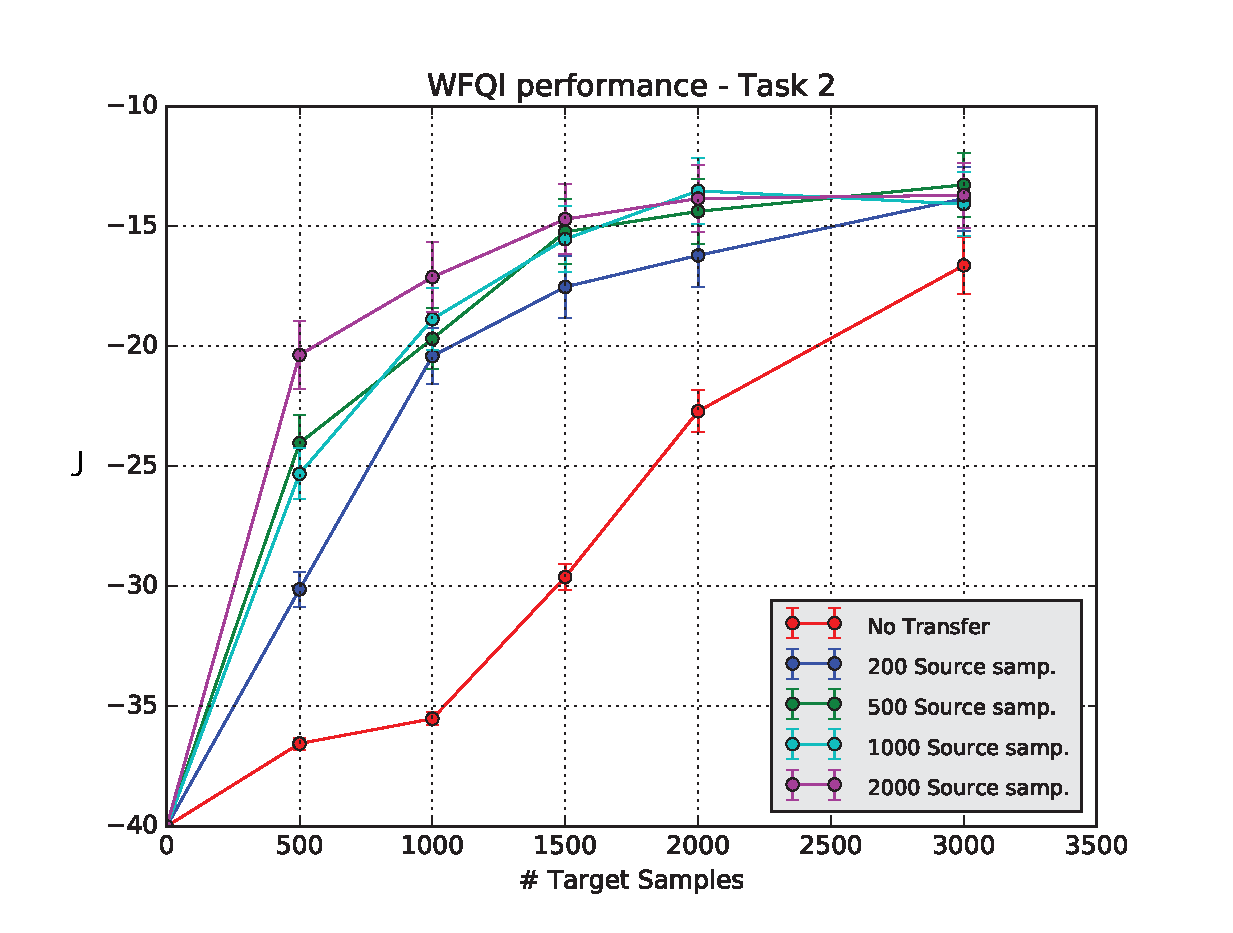
\includegraphics[scale=0.5]{images/WFQIPerf2.eps}
      \caption{WFQI performance Source 2/Target task, est. weights}
      \label{perf2E}
    \end{figure}
    %
    \begin{figure}[H]
      \centering
      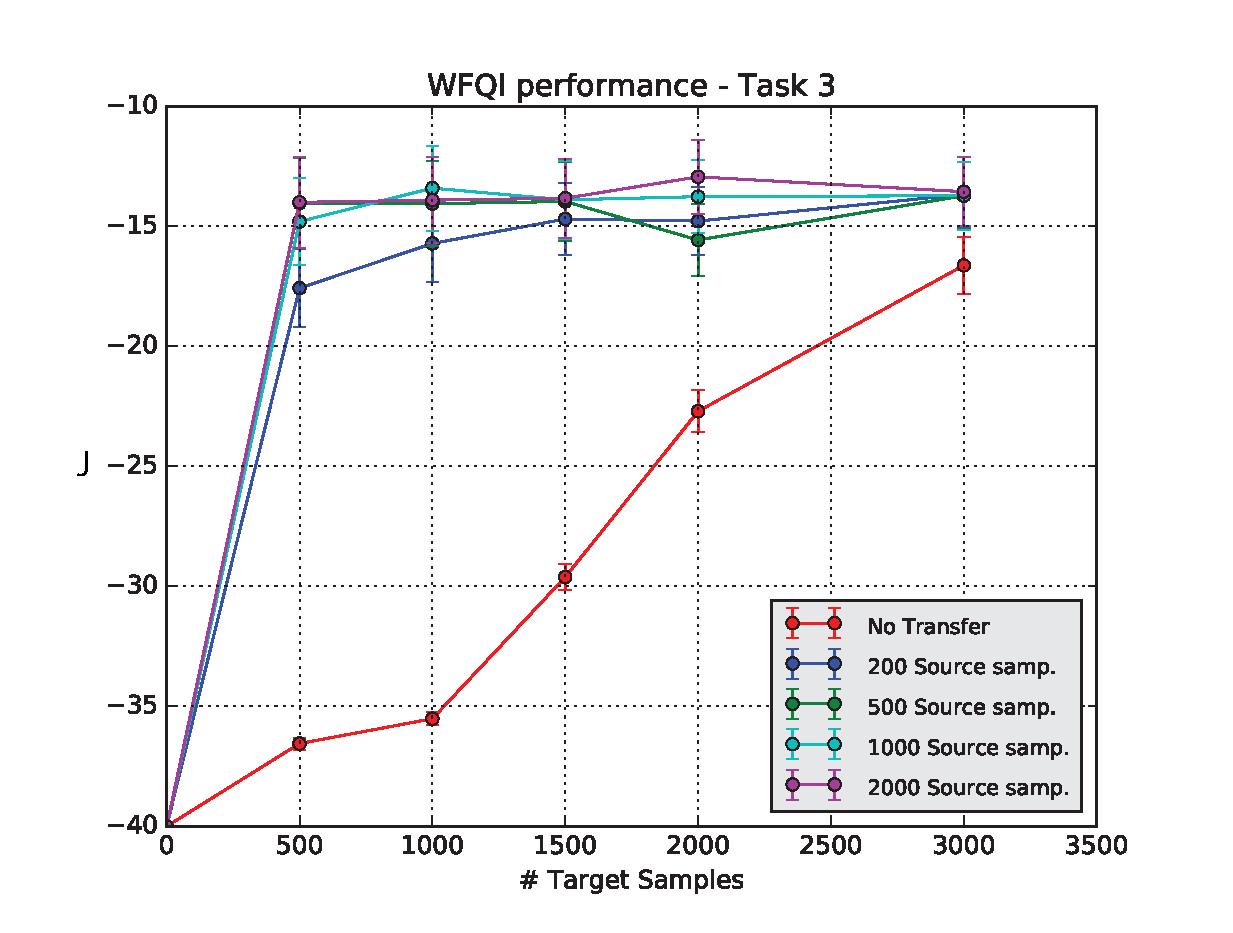
\includegraphics[scale=0.5]{images/WFQIPerf3.eps}
      \caption{WFQI performance Source 3/Target task, est. weights}
      \label{perf3E}
    \end{figure}
    %

    \noindent In this last set of experiments the samples are transferred from all
    the source tasks toward the target in equal quantities.

    \begin{figure}[H]
      \centering
      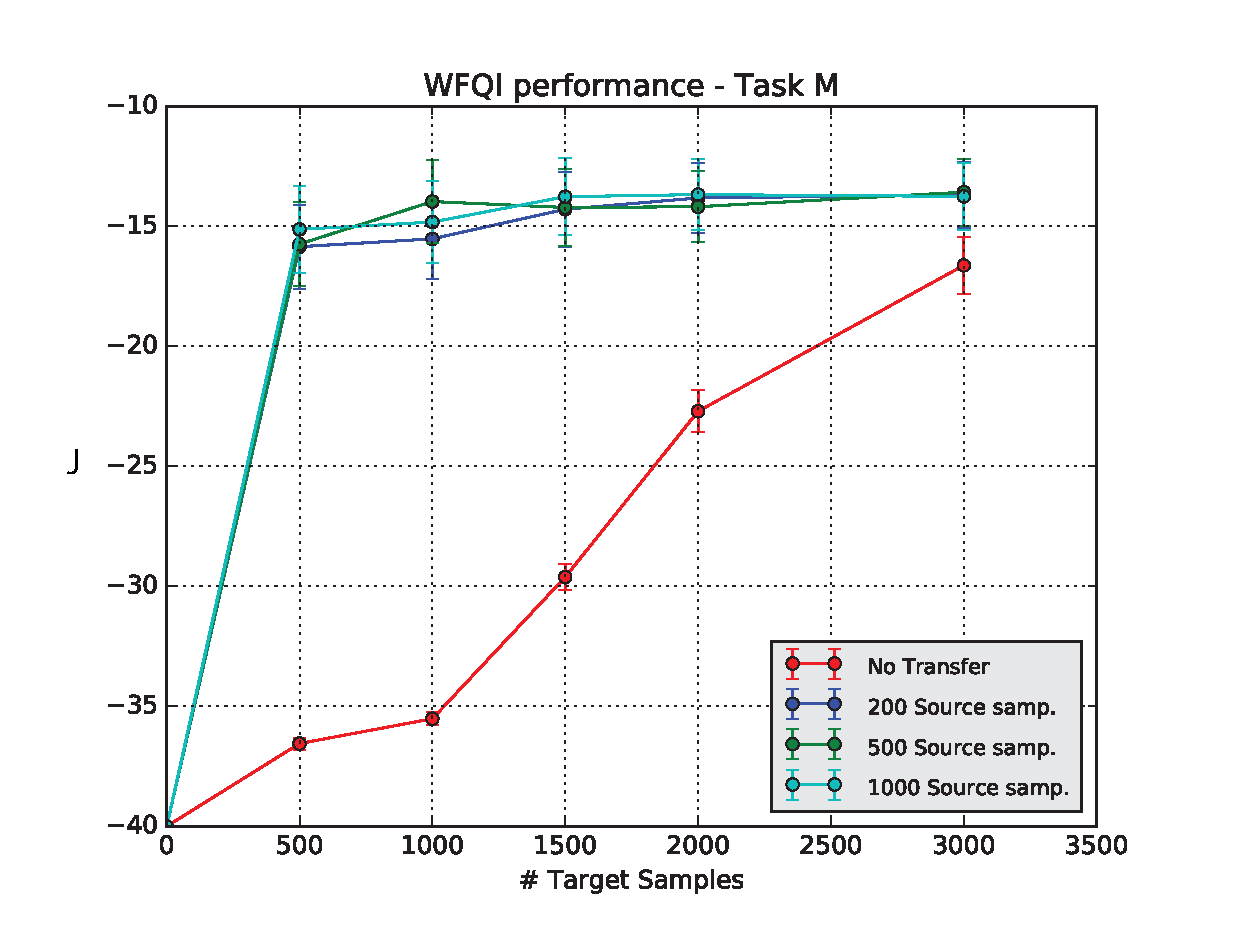
\includegraphics[scale=0.5]{images/WFQIPerfM.eps}
      \caption{WFQI performance Source 1/2/3/Target task, est. weights}
      \label{perfME}
    \end{figure}

    \vspace{3cm}
    %

    \noindent Again he results reflects the theoretical expectation: the best performances are achieved
    with the source tasks 1 and 3, on the other side the source task 2 appear to be of little help.\newline
    Also in this situation our algorithm is able to maintain the ability to successfully
    limit the phenomena of the negative transfer; indeed the performance in figure \ref{perfME}
    seems to not be influenced by the bad sample present in Source task 2.\newline

    \noindent In addition we provide the results obtained using Equation \ref{mean-weight} using
    the correct and an overestimated value for $\sigma^{2}$. The task at hand is very simple but
    we can notice, in the case we do not fake the value of $\sigma^{2}$, a poor performance
    when the number of source samples is low. This effect is due to the fact that when $\sigma_{GP,S}^{2}$
    is high formula \ref{mean-weight} produces a very imprecise estimation of the weights.

    \begin{figure}[H]
      \centering
      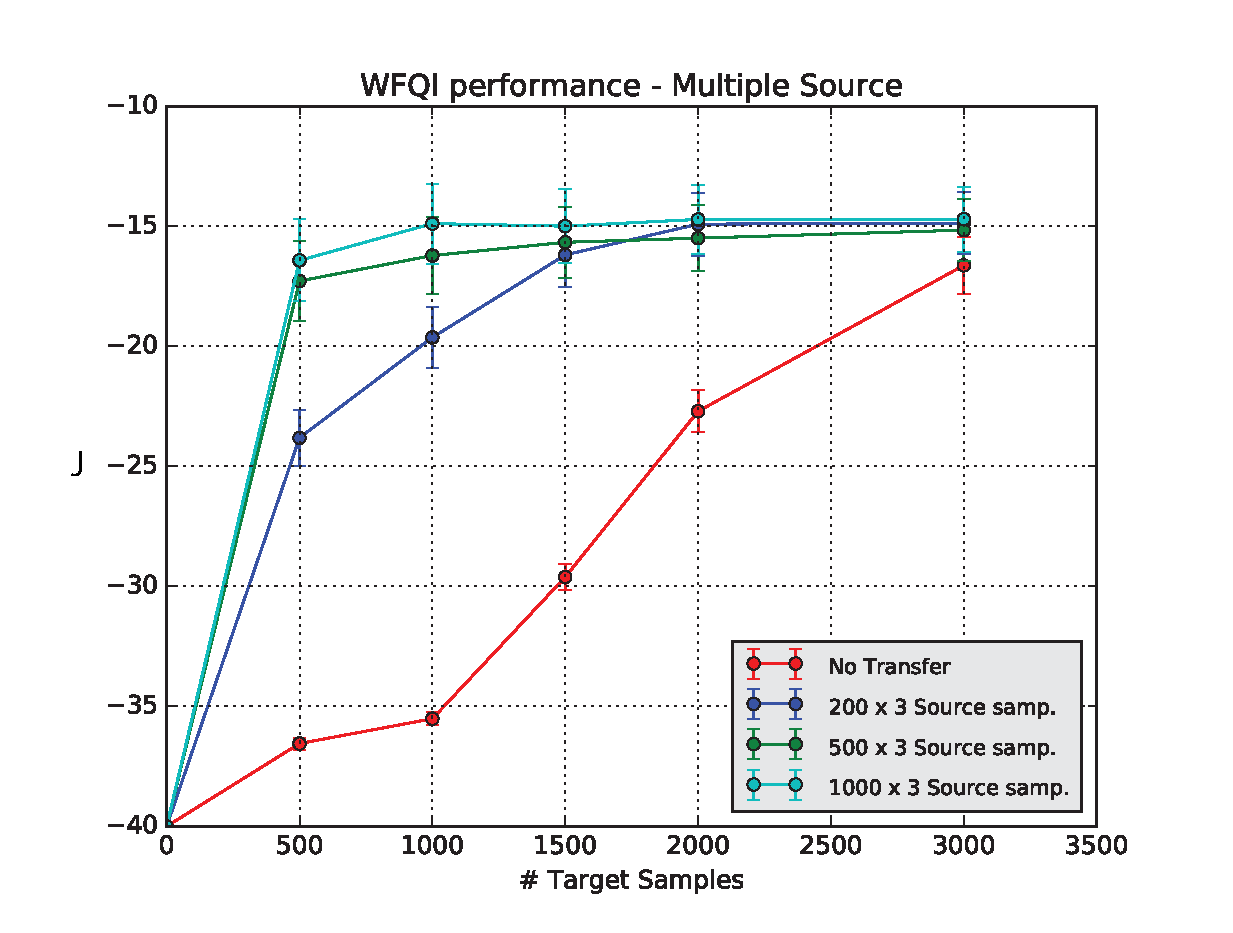
\includegraphics[scale=0.6]{images/WFQIPerfM_V1_MEAN.eps}
      \caption{Performance over Puddle-World V1, no $\sigma^{2}$ overestimation, $\sigma^{2} = 0.01$, multiple source tasks}
      \label{}
    \end{figure}

    \begin{figure}[H]
      \centering
      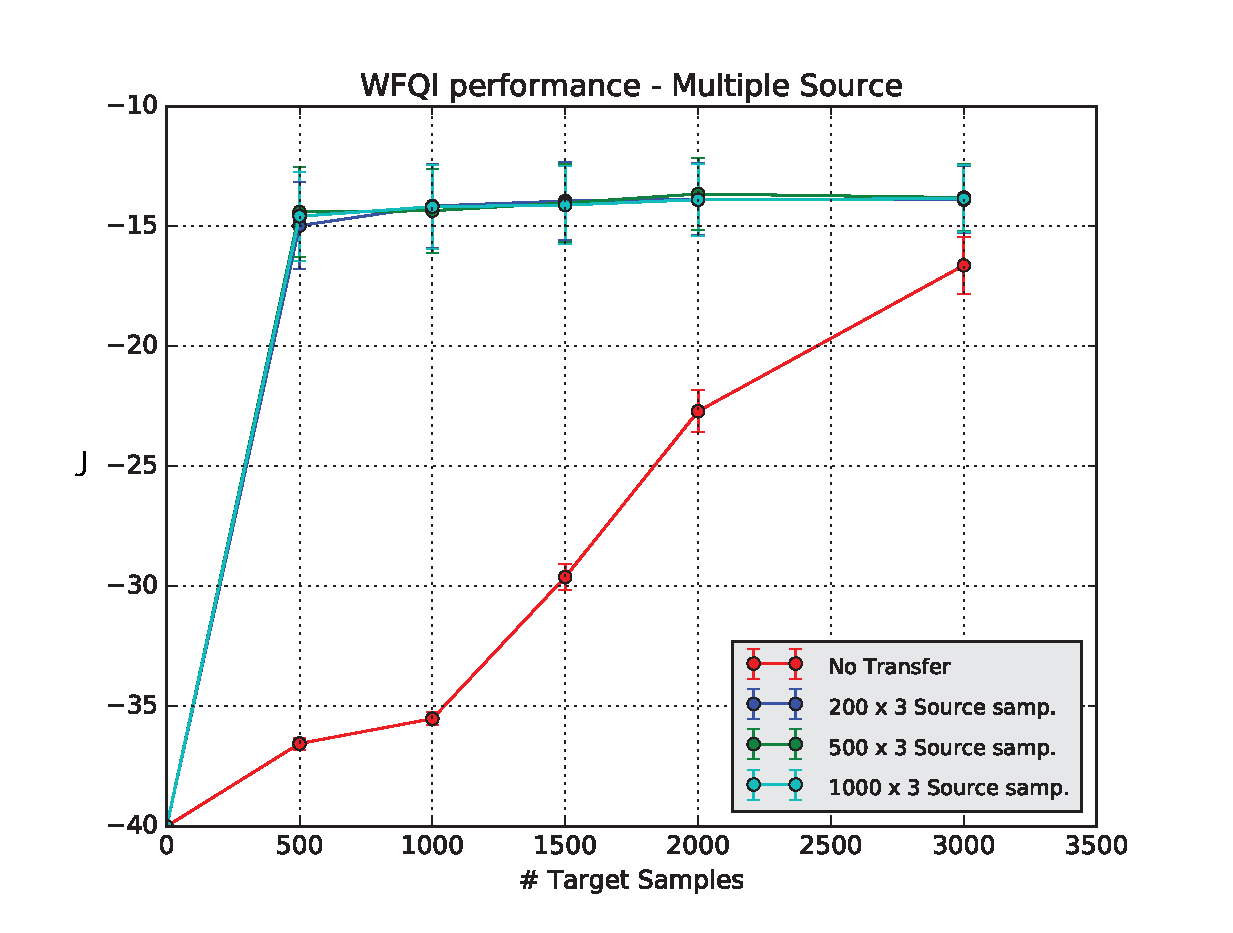
\includegraphics[scale=0.5]{images/WFQIPerfM_V1_MEAN2.eps}
      \caption{Performance over Puddle-World V1, with $\sigma^{2}$ overestimation, $\sigma^{2} = 0.09$, multiple source tasks}
      \label{}
    \end{figure}


    \noindent As a final remark notice that using a weight $w = w_r*w_p$ in this environment would be
    of great disadvantage. Indeed here we assume that the transition model does not change between
    source and target task while the reward model can change arbitrary. This means we can assume
    $w_p = 1$ while the value of $w_r$ can change depending on the specific sample. If the source task
    is significantly different from the target it means that $w$ will assume a low value in the entire
    state-action space thus limiting the transfer. On the other hand with our approach, where reward weights
    are only used in the first iteration and transition weights are used in the remaining, the transfer
    procedure can fully exploit the similarities of the dynamics and thus maximizes the number of transferred
    samples.


  \section{Results - Puddle World Version 2}
    \noindent This environment is a variation of the previous puddle world, in this scenario when the agent is
    close to a puddle in addition to the reward penalty it also modifies its step length that decreases
    proportionally to the distance with respect to the center of the puddle. This situation is much more
    complicated from the transfer perspective: in addition to the weight necessary for the reward model, in
    this case we need to compute a weight also for the transfer of the dynamics of the agent (that now are
    changed).

    \subsection{Ideal Weights}
    \noindent In the first set of experiments we test the performance of WFQI using the ideal weights,
    that is we assume to perfectly know the stochastic model for both the reward and transition model.
    As expected we obtain over the single task transfer an almost perfect performance, meaning that also
    with a very small amount of transferred source samples we reach the score achieved by the optimal policy.\newline

    \noindent The parameters for the tree-based WFQI algorithm are: 50 estimators, 2 random splits and 1 minimum samples per leaf.

    \begin{figure}[H]
      \raggedbottom
      \centering
      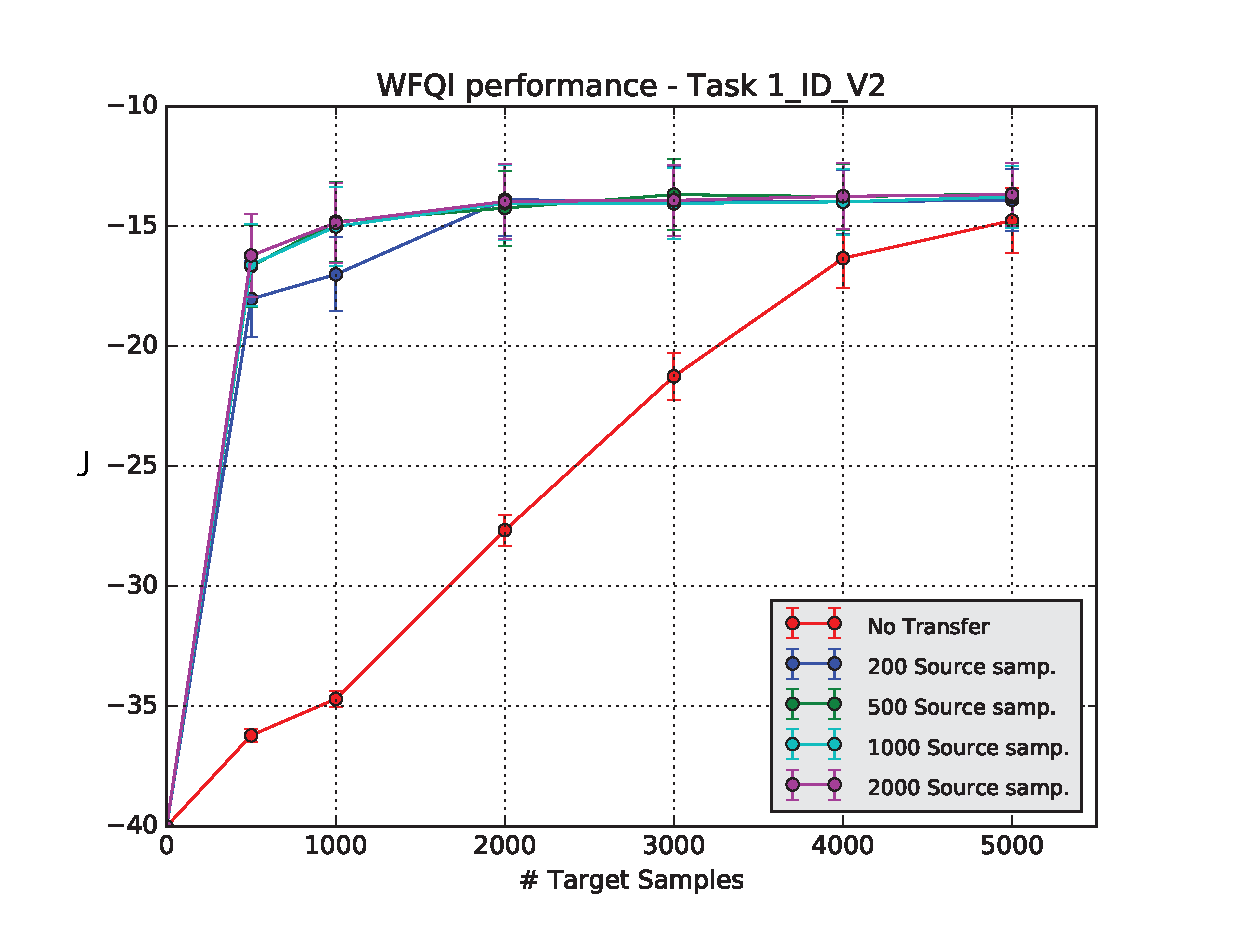
\includegraphics[scale=0.5]{images/WFQIPerf1_ID_V2.eps}
      \caption{WFQI performance Source 1/Target task, ideal weights}
      \label{perf1E}
    \end{figure}
    %
    \begin{figure}[H]
      \raggedbottom
      \centering
      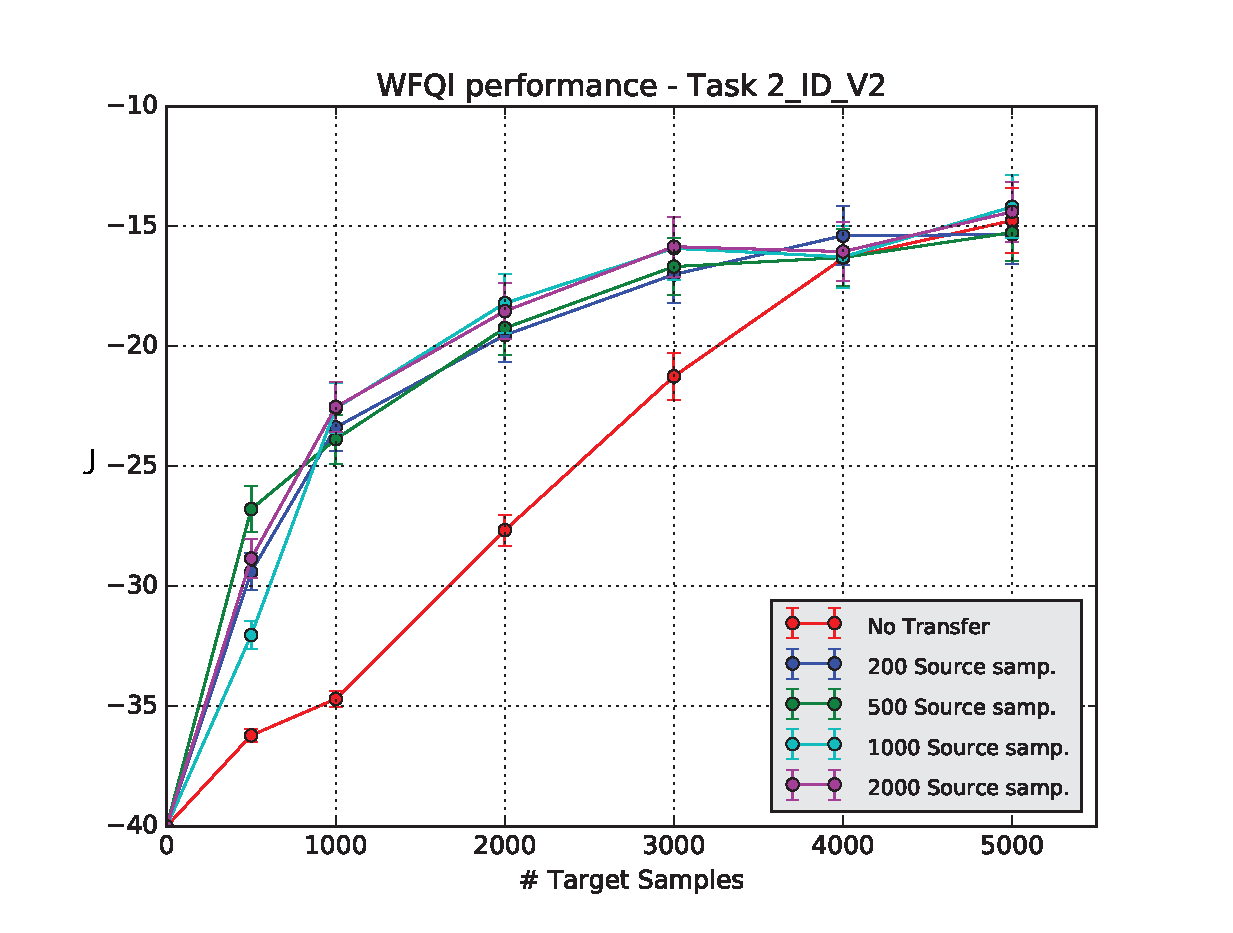
\includegraphics[scale=0.5]{images/WFQIPerf2_ID_V2.eps}
      \caption{WFQI performance Source 2/Target task, ideal weights}
      \label{perf2E}
    \end{figure}
    %
    \begin{figure}[H]
      \raggedbottom
      \centering
      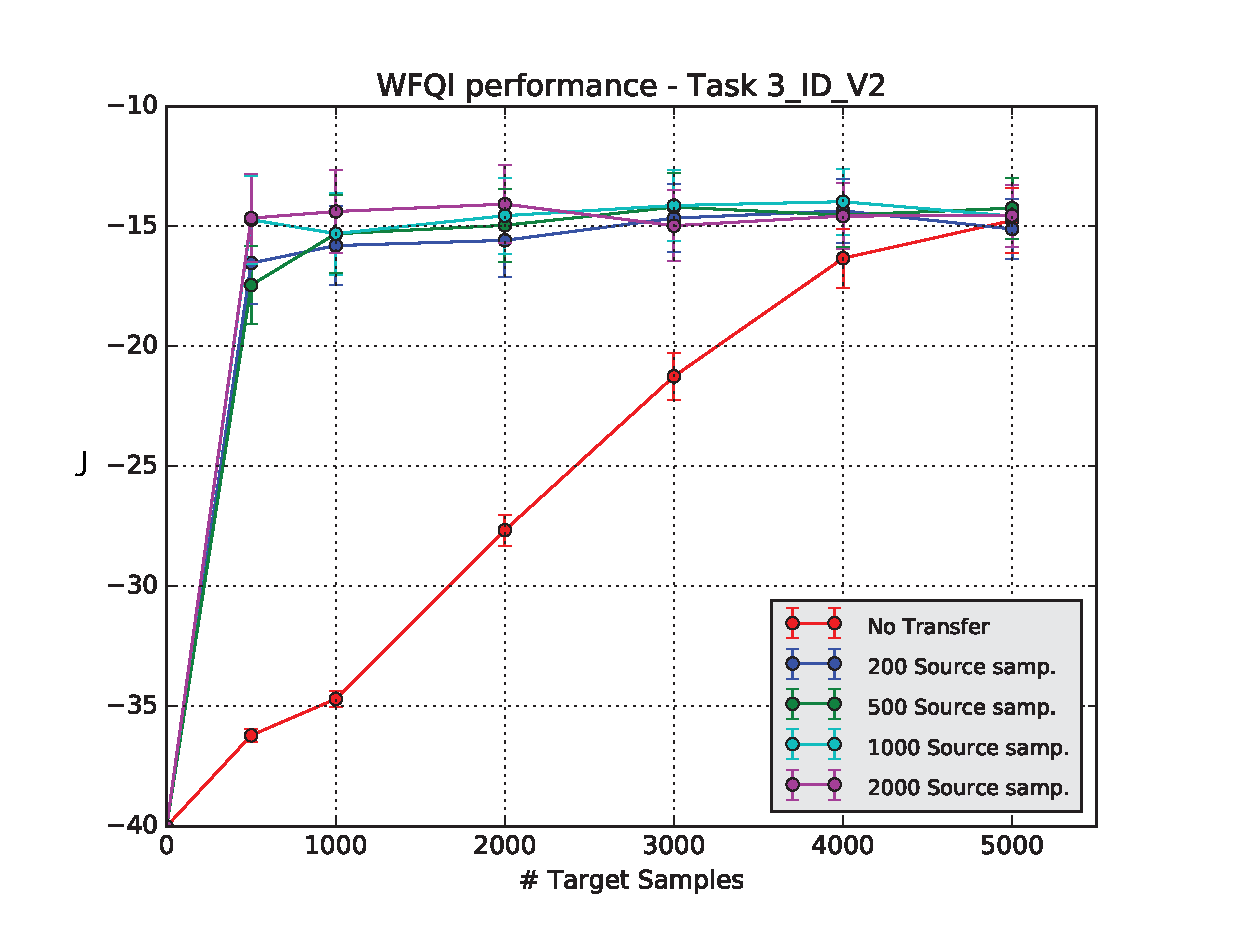
\includegraphics[scale=0.5]{images/WFQIPerf3_ID_V2.eps}
      \caption{WFQI performance Source 3/Target task, ideal weights}
      \label{perf3E}
    \end{figure}
    %

    \noindent In this last set of experiments the samples are transferred from all
    the source tasks toward the target in equal quantities. Again we highlight the
    fact that despite the fact that samples coming from the second source task
    are not effective for the transfer, the algorithm is able to completely
    eliminate the negative transfer and to reach the maximum performance.

    \begin{figure}[H]
      \raggedbottom
      \centering
      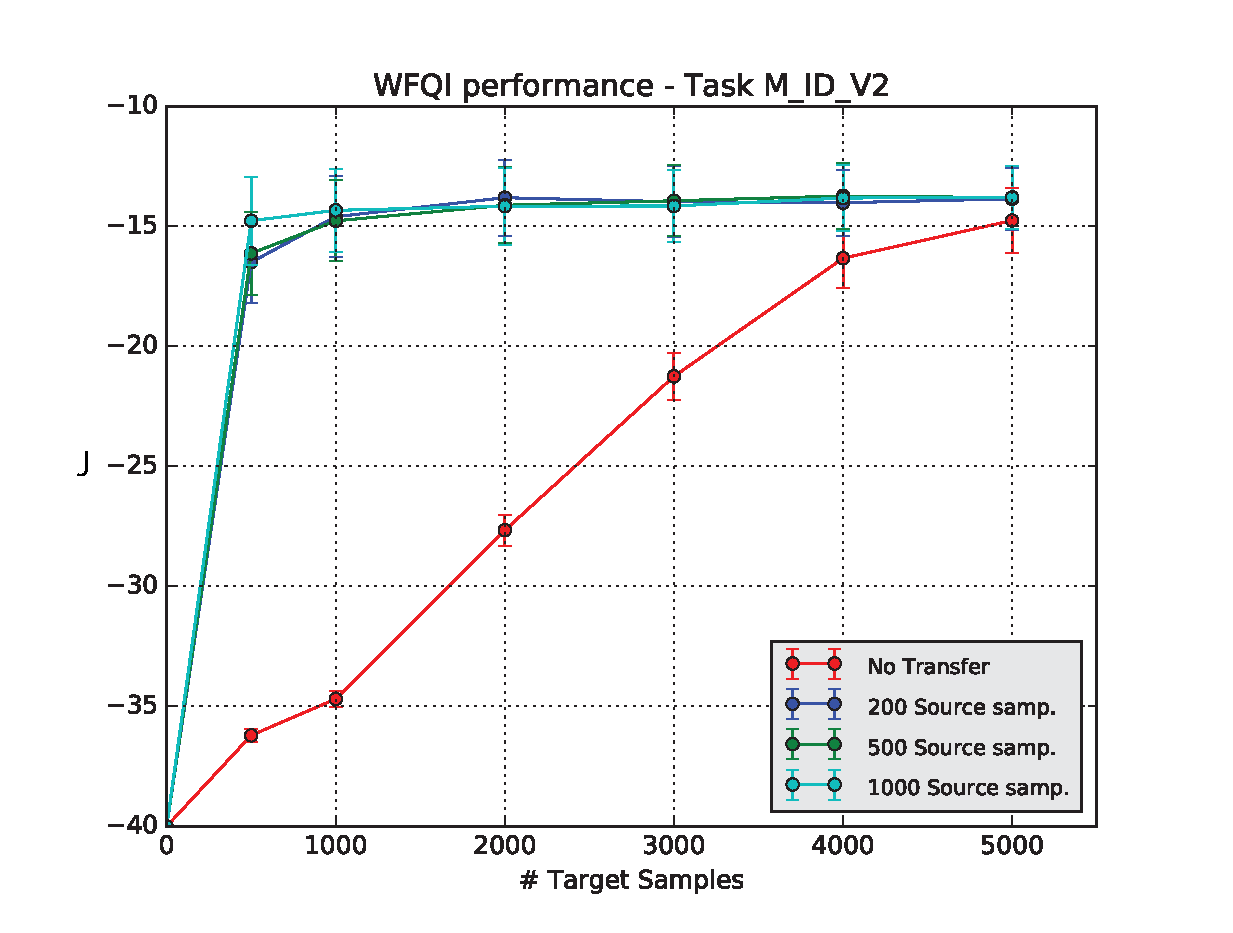
\includegraphics[scale=0.5]{images/WFQIPerfM_ID_V2.eps}
      \caption{WFQI performance Source 1/2/3/Target task, ideal weights}
      \label{perfMIDV2}
    \end{figure}
    %

    \subsection{Estimated Weights}

    \noindent For this set of experiments weights are calculated
    using algorithms \ref{rw_weight_est} and \ref{rw_transition_est}. These algorithms provide only an
    estimation of the real weights, therefore the use of the corresponding source samples in the target
    task is not perfectly unbiased (as in the previous scenario). The performance is not as good as
    in the ideal case due to the error introduced thanks to the estimation of the weights.
    Weights are estimated according to Equation \ref{eur}.

    \begin{figure}[H]
      \raggedbottom
      \centering
      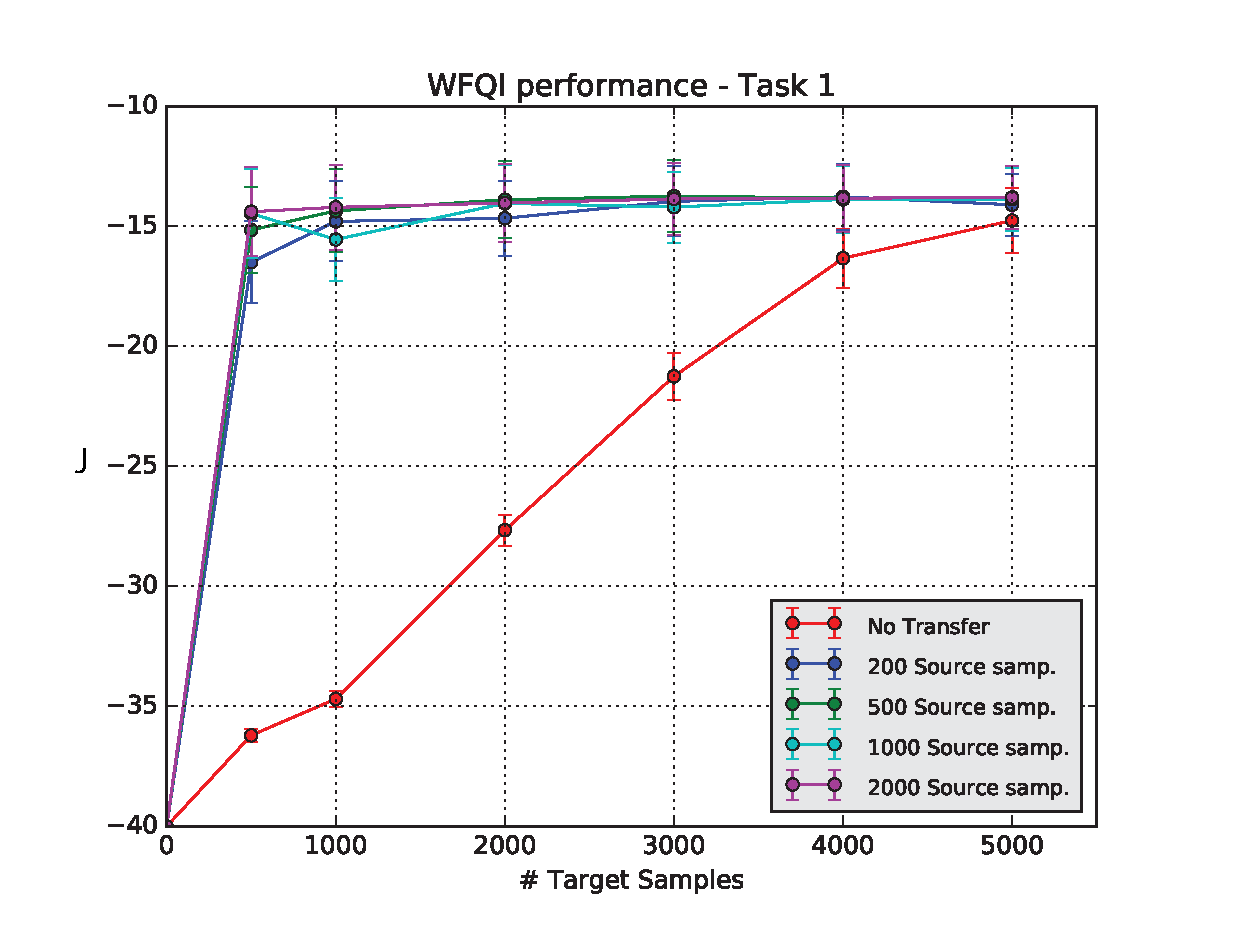
\includegraphics[scale=0.5]{images/WFQIPerf1_V2.eps}
      \caption{WFQI performance Source 1/Target task, est. weights}
      \label{perf1V2}
    \end{figure}
    %

    \begin{figure}[H]
      \raggedbottom
      \centering
      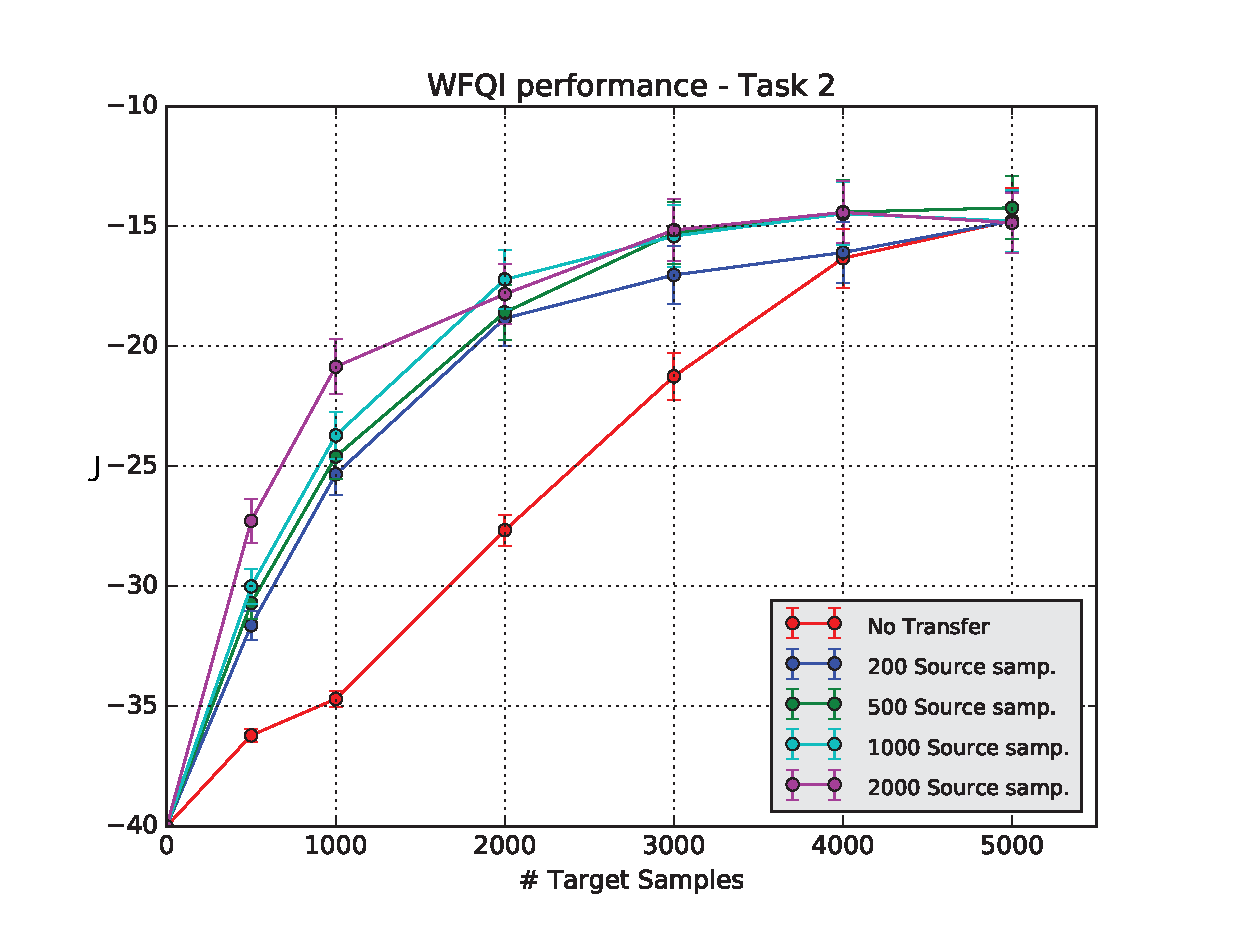
\includegraphics[scale=0.5]{images/WFQIPerf2_V2.eps}
      \caption{WFQI performance Source 2/Target task, est. weights}
      \label{perf2V2}
    \end{figure}
    %

    \begin{figure}[H]
      \raggedbottom
      \centering
      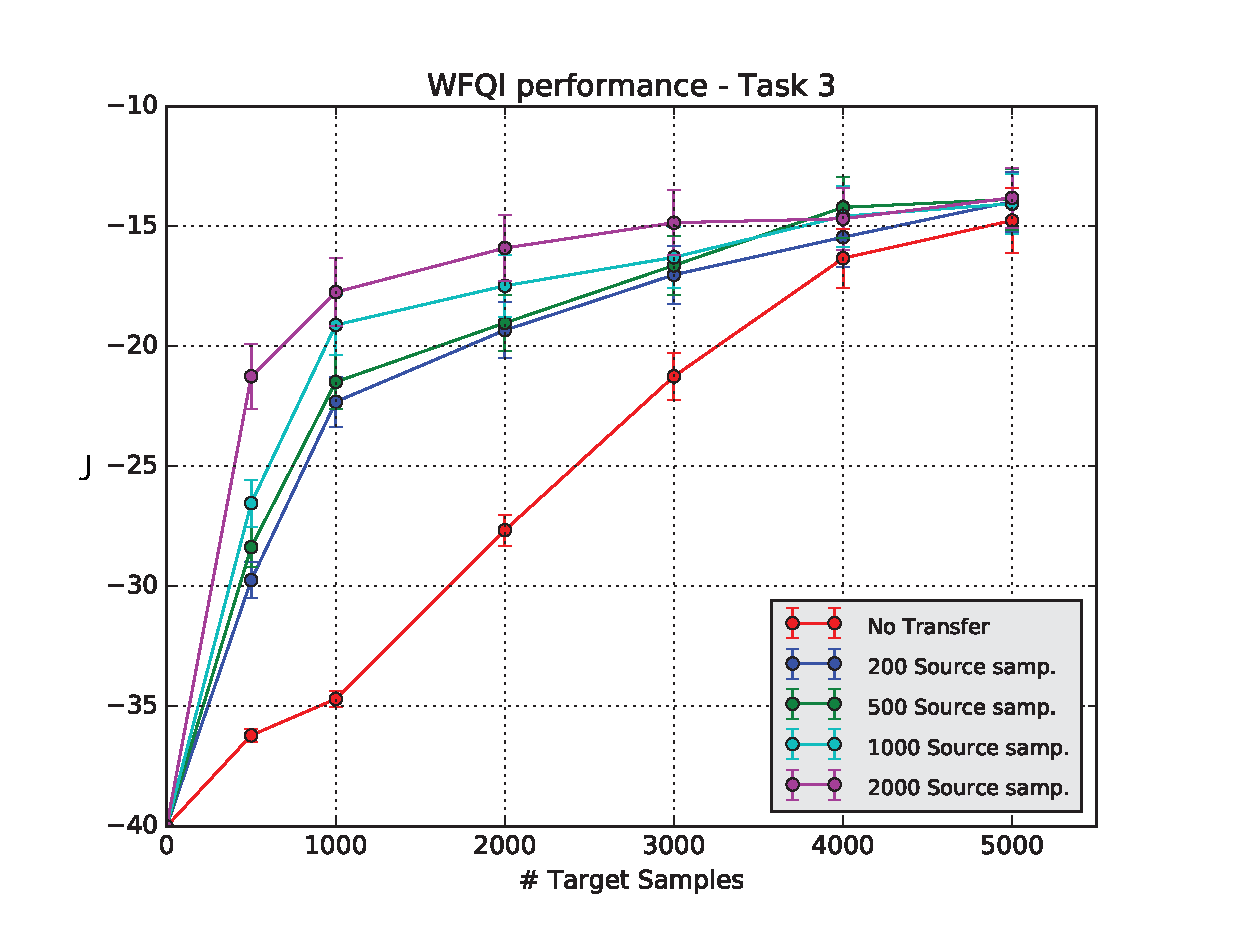
\includegraphics[scale=0.5]{images/WFQIPerf3_V2.eps}
      \caption{WFQI performance Source 3/Target task, est. weights}
      \label{perf3V2}
    \end{figure}
    %

    \noindent In this last set of experiments the samples are transferred from all
    the source tasks toward the target in equal quantities. Also in this case,
    despite the fact that samples coming from the second source task
    are not effective for the transfer, the algorithm is able to eliminate the negative
    transfer effect and to achieve an satisfactory performance.

    \begin{figure}[H]
      \raggedbottom
      \centering
      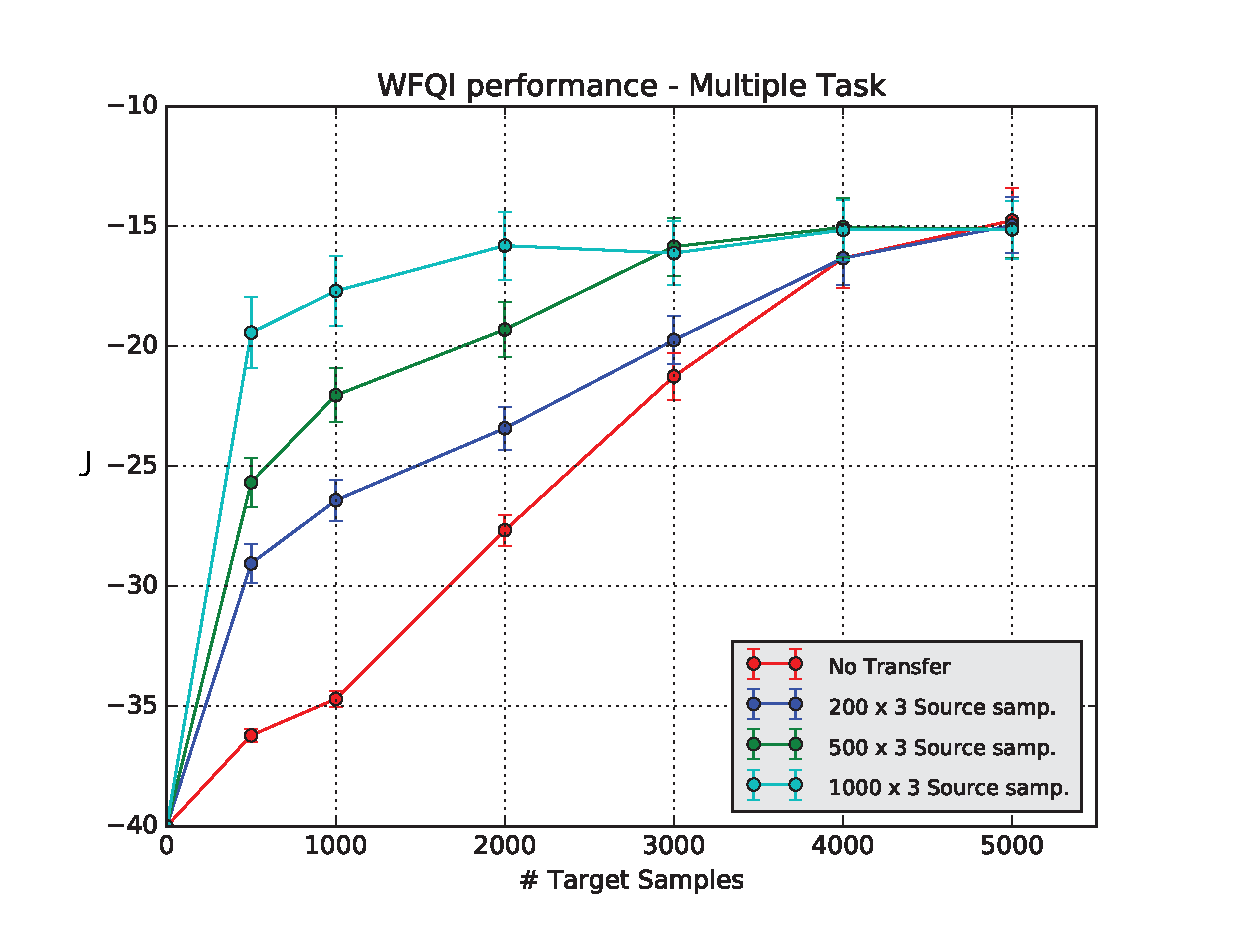
\includegraphics[scale=0.5]{images/WFQIPerfM_V2.eps}
      \caption{WFQI performance Source 1/2/3/Target task, est. weights}
      \label{perfMV2}
    \end{figure}

    \noindent In addition we also report the results when weights are estimated according to
    Formula \ref{mean-weight} using respectively, in Figure \ref{mean-res1} $\sigma^{2}_r = 0.01$ and
    $\sigma^{2}_{p} = 0.04$ and in Figure \ref{mean-res2} $\sigma^{2}_{r} = 0.09$ and $\sigma^{2}_{p} = 0.36$.

    \begin{figure}[H]
      \centering
      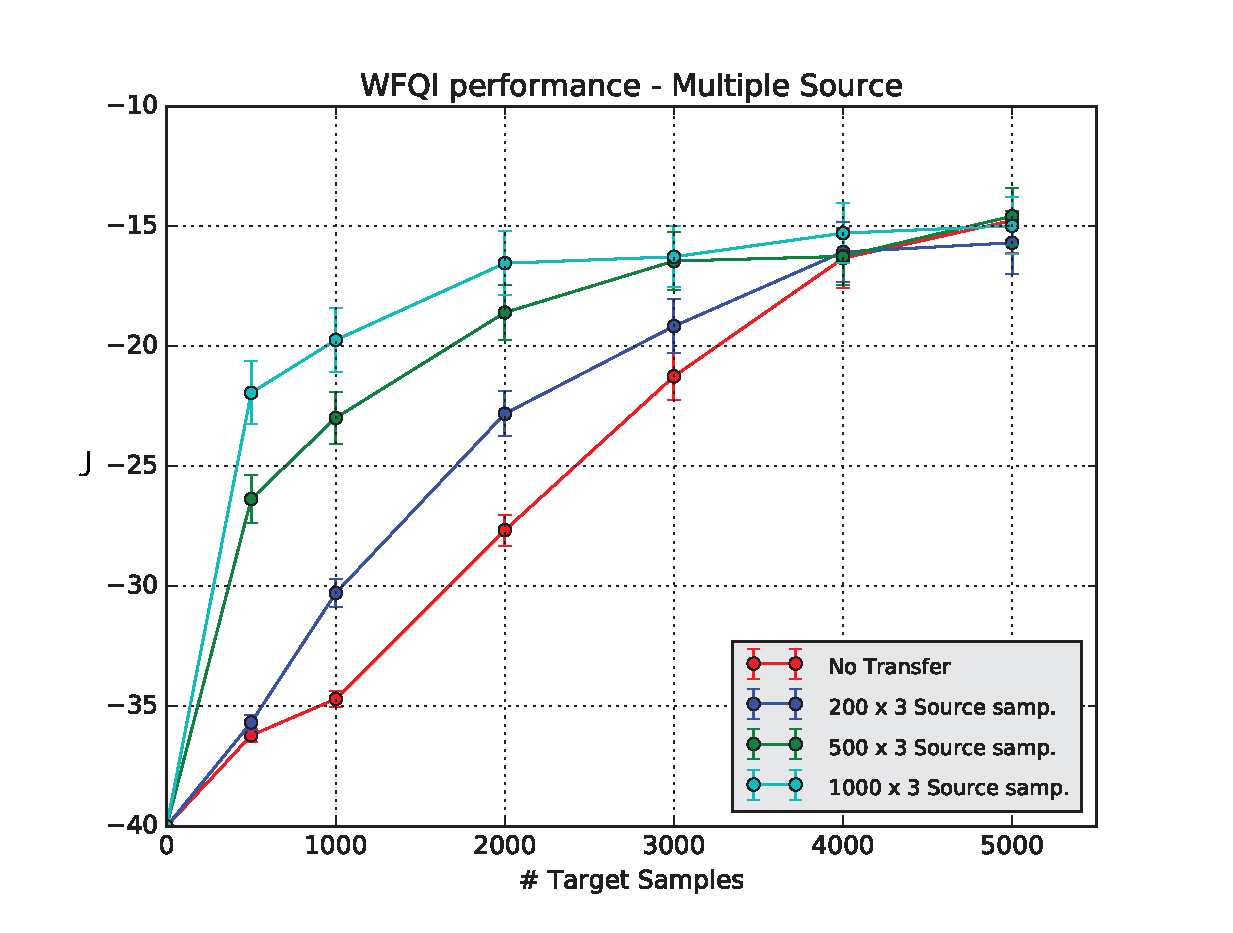
\includegraphics[scale=0.5]{images/WFQIPerfM_V2_MEAN.eps}
      \caption{Puddle-World performance, multiple source tasks, Equation \ref{mean-weight} \textbf{without} $\sigma^{2}$ overestimation}
      \label{mean-res1}
    \end{figure}

    \begin{figure}[H]
      \centering
      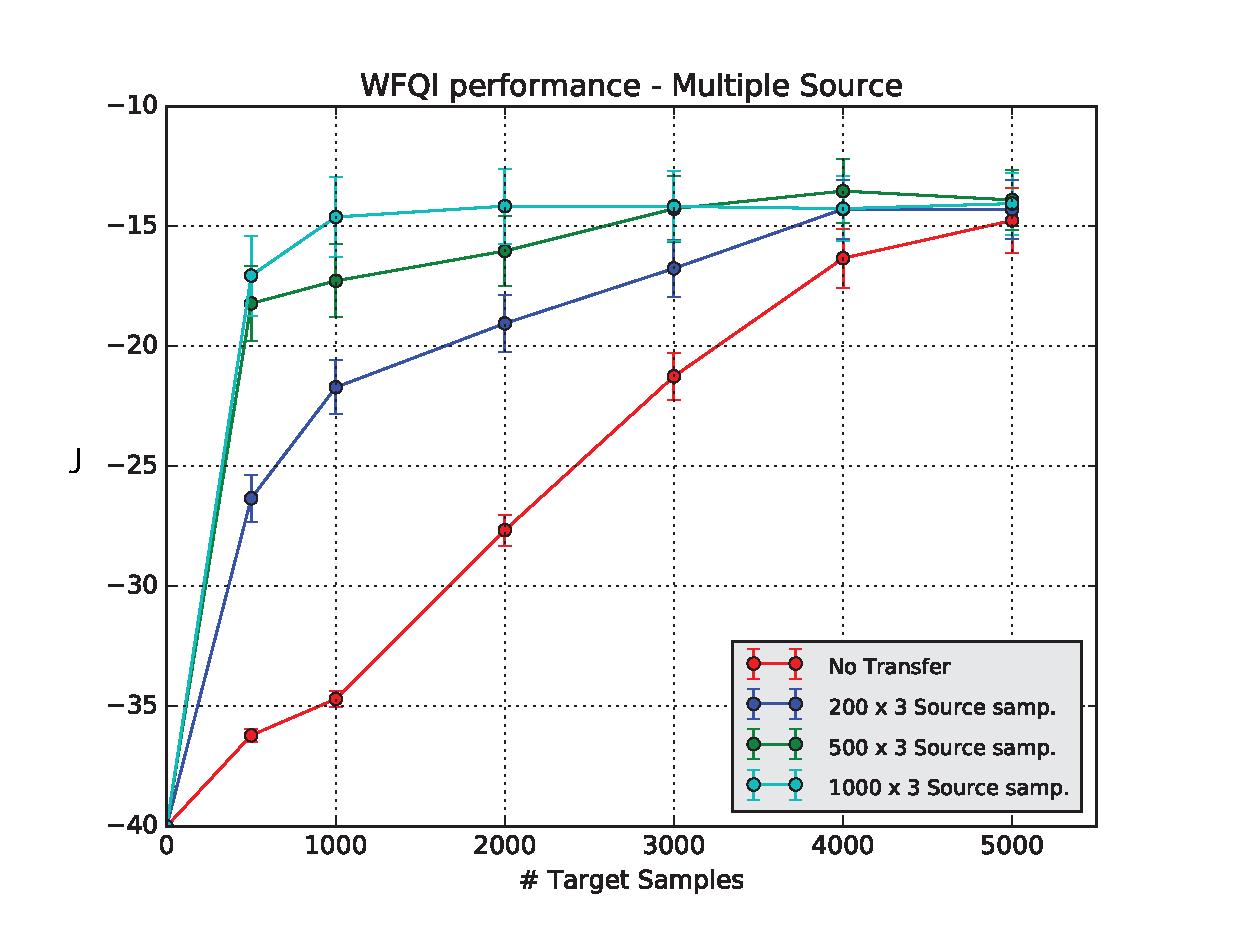
\includegraphics[scale=0.5]{images/WFQIPerfM_V2_MEAN2.eps}
      \caption{Puddle-World performance, multiple source tasks, Equation \ref{mean-weight} \textbf{with} $\sigma^{2}$ overestimation}
      \label{mean-res2}
    \end{figure}


    \noindent We observe, in the first case, poor performances, mainly due high number of discarded samples.
    In the second graph we notice a much better performance due to the overestimation of $\sigma^{2}$ for
    both reward and transition model, in this case even better than the heuristic approach.
    %

  \section{Acrobot Environment}
    \noindent Acrobot is a two-link underactuated robot, we refer to the model described by \cite{ernst2005tree}. A
    graphical representation is depicted in figure \ref{acrobot_fig}.

    \begin{figure}[H]
      \raggedbottom
      \centering
      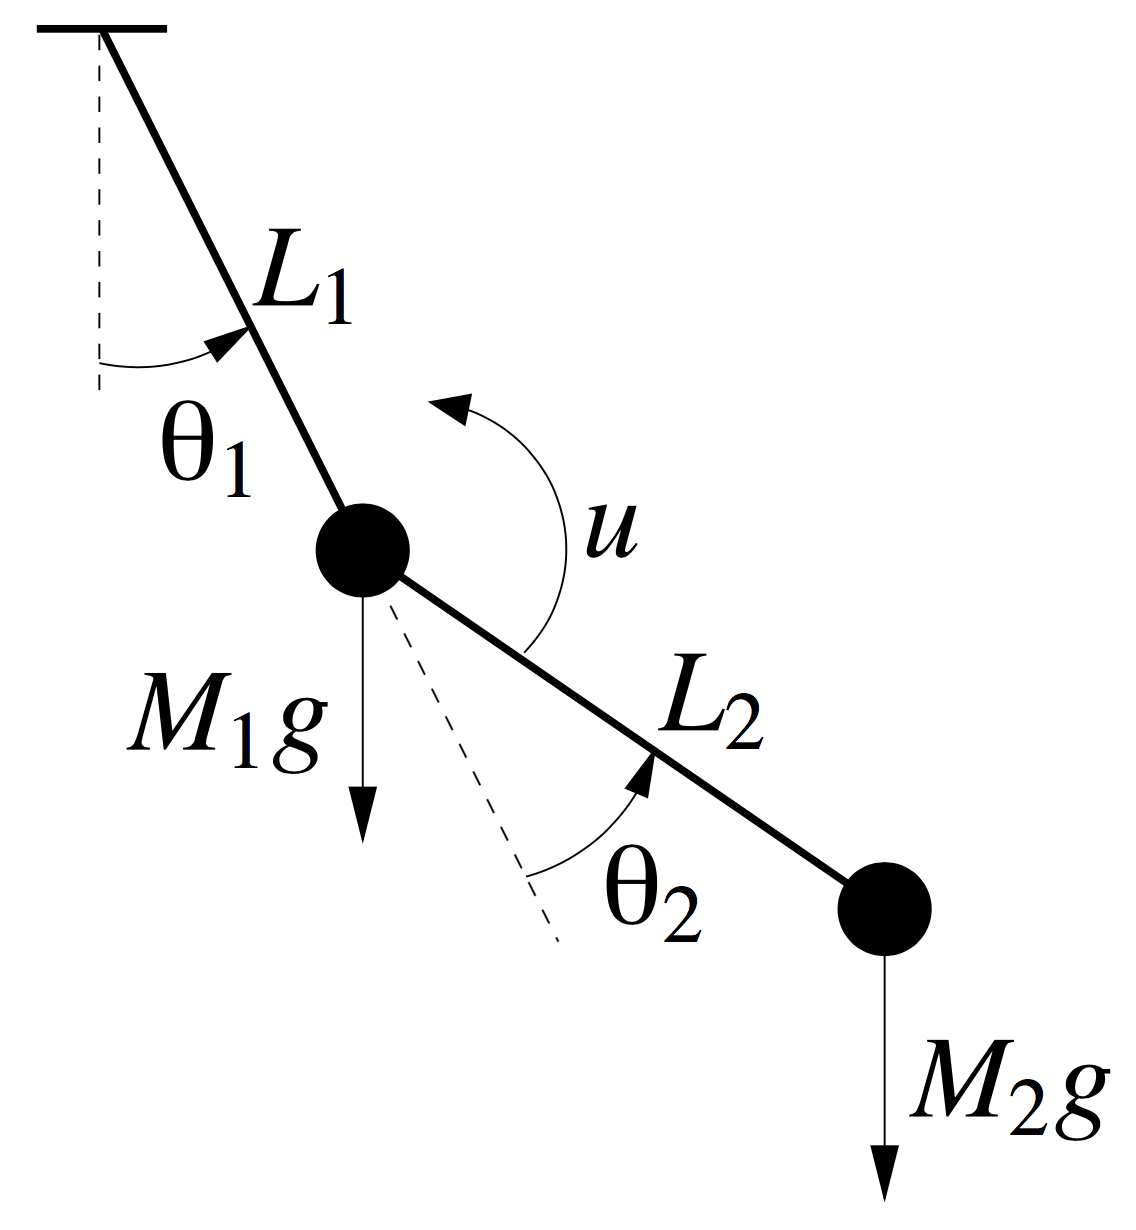
\includegraphics[scale=0.3]{images/acrobot.png}
      \caption{A graphical representation of the Acrobot environment}
      \label{acrobot_fig}
    \end{figure}
    %

    \noindent The state space of the problem is continuous and described by the
    tuple $[\theta_1, \theta_2, \dot{\theta}_1, \dot{\theta}_2]$, where $\theta_1$ and
    $\theta_2$ are the angles of the two links and $\dot{\theta}_1$ and $\dot{\theta}_2$
    are the two corresponding angular speeds. The action space is discrete and the only
    two possibility are to apply a torque of either $-5$ or $5$.\newline
    The goal is to bring as fast as possible the two links in the upright position.
    The reward signal is $-1$ for every action and $0$ when the two links are in the
    neighbourhood of the goal position.\newline

    \noindent The dynamical system equations of the Acrobot are given by:
    \begin{equation}
      \begin{cases}
        d_{11}\ddot{\theta}_1 + d_{12}\ddot{\theta}_2 + c_1 + \phi_1 = -\mu_{1} \dot{\theta}_1 \\
        d_{12}\ddot{\theta}_1 + d_{22}\ddot{\theta}_2 + c_2 + \phi_2 = u - \mu_{2} \dot{\theta}_2 \\
        d_{11} = M_{1}L_{1}^{2} + M_{2}(L_{1}^{2} + L_{2}^{2}  + 2L_{1}L_{2}\cos(\theta_2)) \\
        d_{22} = M_{2}L_{2}^{2} \\
        d_{12} = M_{2}(L_{2}^{2} + 2L_{1}L_{2}\cos{\theta_2}) \\
        c_{1} = -M_{2}L_{1}L_{2}\dot{\theta}_{2}(2\dot{\theta}_{1} + \dot{\theta}_{2})\sin({\theta_2)} \\
        c_{2} = M_{2}L_{1}L_{2}\dot{\theta}_{1}^{2}\sin(\theta_{2}) \\
        \phi_{1} = -(M_{1}L_{1} + M_{2}L_{1}) g \sin(\theta_1) - M_{2}L_{2} g \sin(\theta_1 + \theta_2) \\
        \phi_{2} = -M_{2}L_{2} g \sin(\theta_1 + \theta_2) \\
      \end{cases}
    \end{equation}

    \noindent $g = 9.81 m/s^{2}$ is the gravitational acceleration coefficient while $\mu_1$ and $\mu_2$ are the
    friction coefficients for the corresponding two joints.\newline
    The discount factor $\gamma$ of the corresponding MDP is $0.95$.

    \subsection{Tasks}
      \noindent For the Target task we set $L_1 = 1.0, L_2 = 1.0, M_1 = 1.0, M_2 = 1.0, \mu_1 = 0.1, \mu_2 = 0.1$.\newline
      For the Source task 1 we set $L_1 = 0.9, L_2 = 0.95, M_1 = 0.95, M_2 = 1.0, \mu_1 = 0.1, \mu_2 = 0.1$\newline
      For the Source task 2 we set $L_1 = 0.8, L_2 = 0.6, M_1 = 0.9, M_2 = 1.0, \mu_1 = 0.1, \mu_2 = 0.1$\newline
      For the Source task 3 we set $L_1 = 0.85, L_2 = 0.85, M_1 = 0.9, M_2 = 0.9, \mu_1 = 0.1, \mu_2 = 0.1$\newline

      \noindent Tests are performed singularly, $Source \rightarrow Target$ and in ensemble, $Source 1/2/3 \rightarrow Target$.

    \vspace{10cm}
    \subsection{Results - Acrobot}
    \noindent In this section we report the results relative to the Acrobot environment, tests are performed with the following
    parameters: $Estimators = 50, Random Split = 5, Min. Samples per leaf = 2$, WFQI is executed over 50 iterations,
    the horizon of the MDP is set to 100. Results are averaged of 30 runs.\newline
    It is important to observe the these settings represents a much more difficult than the previous
    experiments: we are no more in a gaussian settings (while in Puddle World the dynamics and rewards models are
    assumed to be normally distributed), this means that the use of GPs introduces a further error (in addition
    to the bias of the estimated weights); despite this further difficulty again we are able to obtain interesting
    advantages from our approach. Weights are estimate according to Equation \ref{eur}.

    \begin{figure}[H]
      \raggedbottom
      \centering
      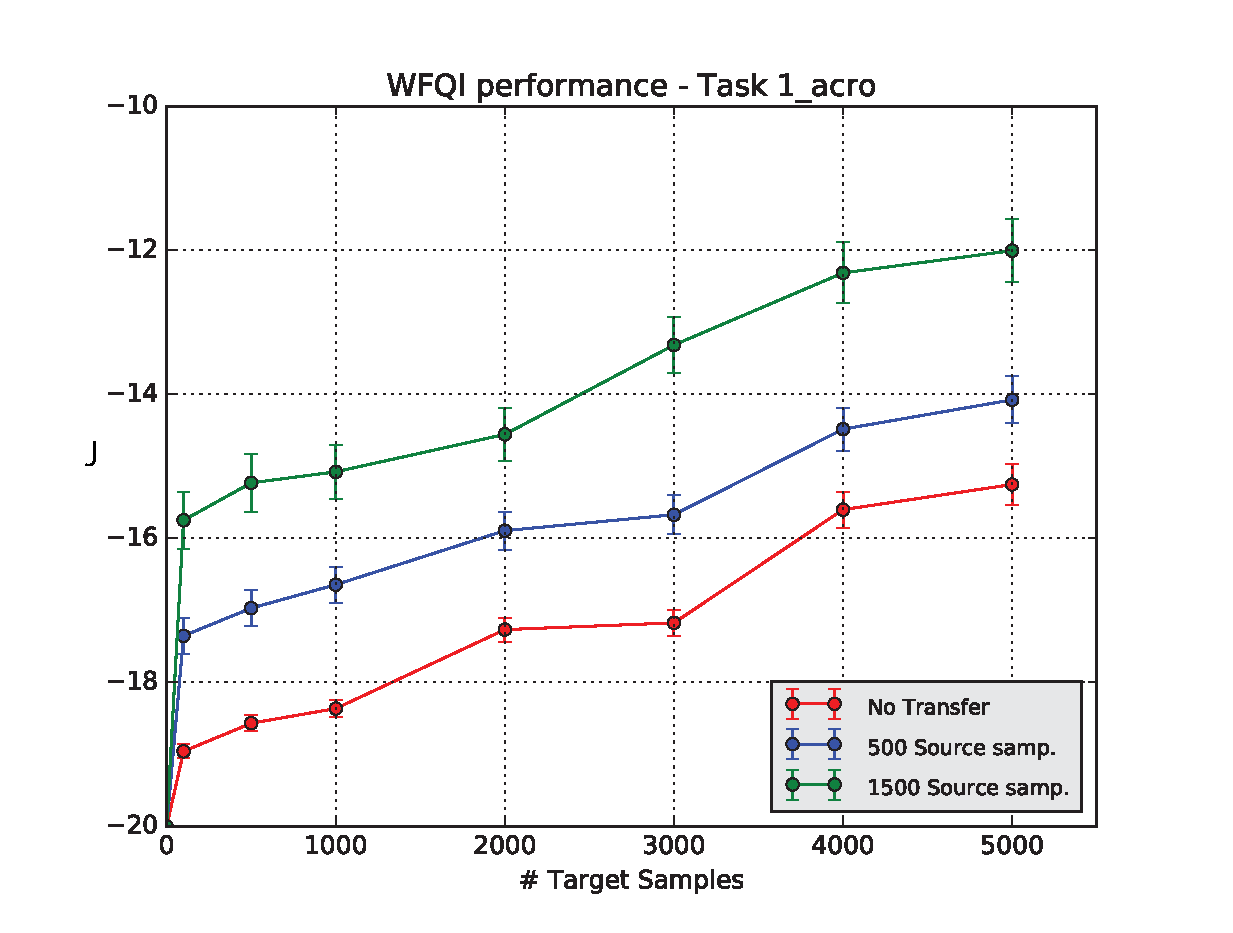
\includegraphics[scale=0.5]{images/WFQIPerf1_acro.eps}
      \caption{WFQI performance Source 1/Target task, est. weights}
      \label{acro1}
      %
    \end{figure}
    \begin{figure}[H]
      \raggedbottom
      \centering
      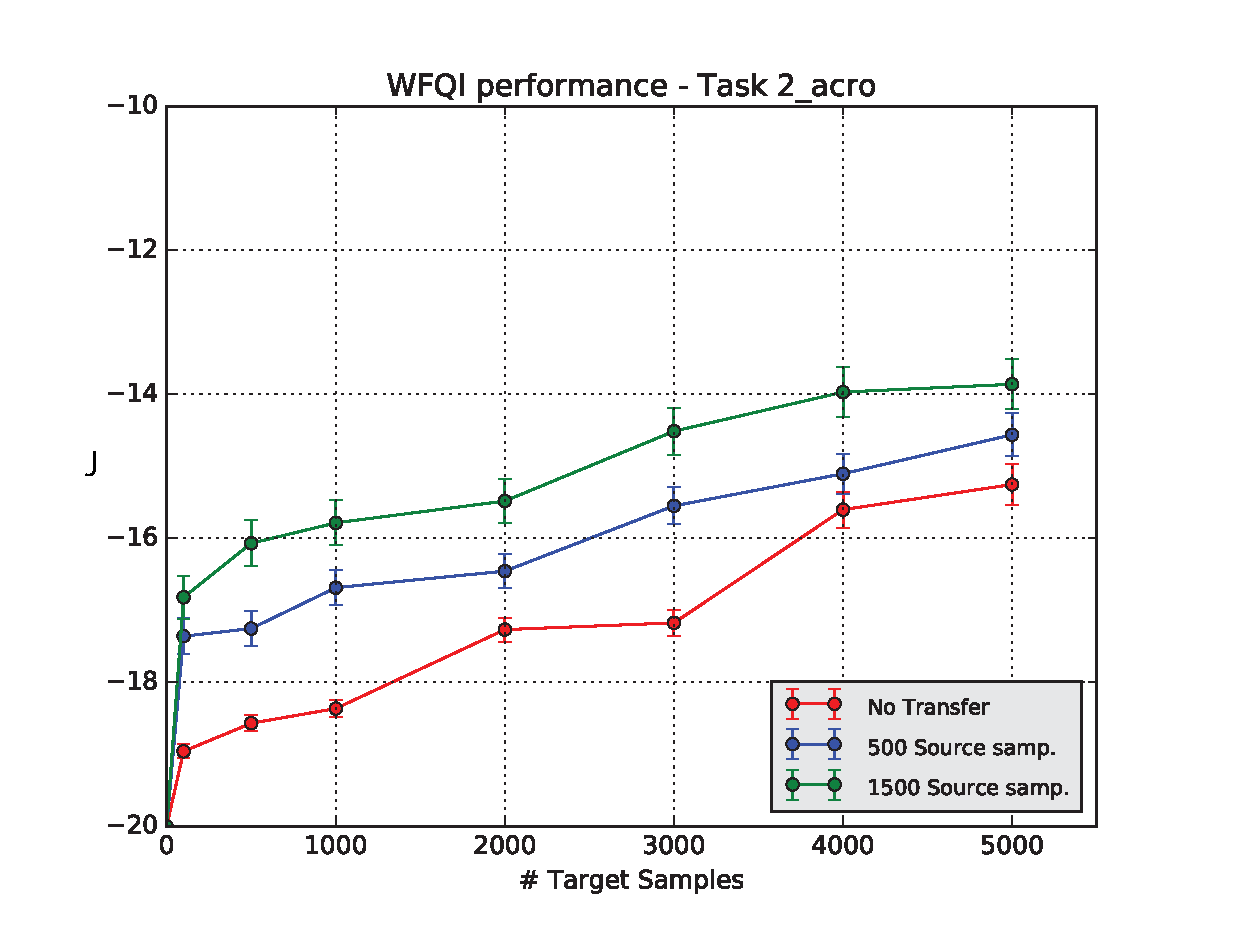
\includegraphics[scale=0.5]{images/WFQIPerf2_acro.eps}
      \caption{WFQI performance Source 2/Target task, est. weights}
      \label{acro2}
      %
    \end{figure}
    \begin{figure}[H]
      \raggedbottom
      \centering
      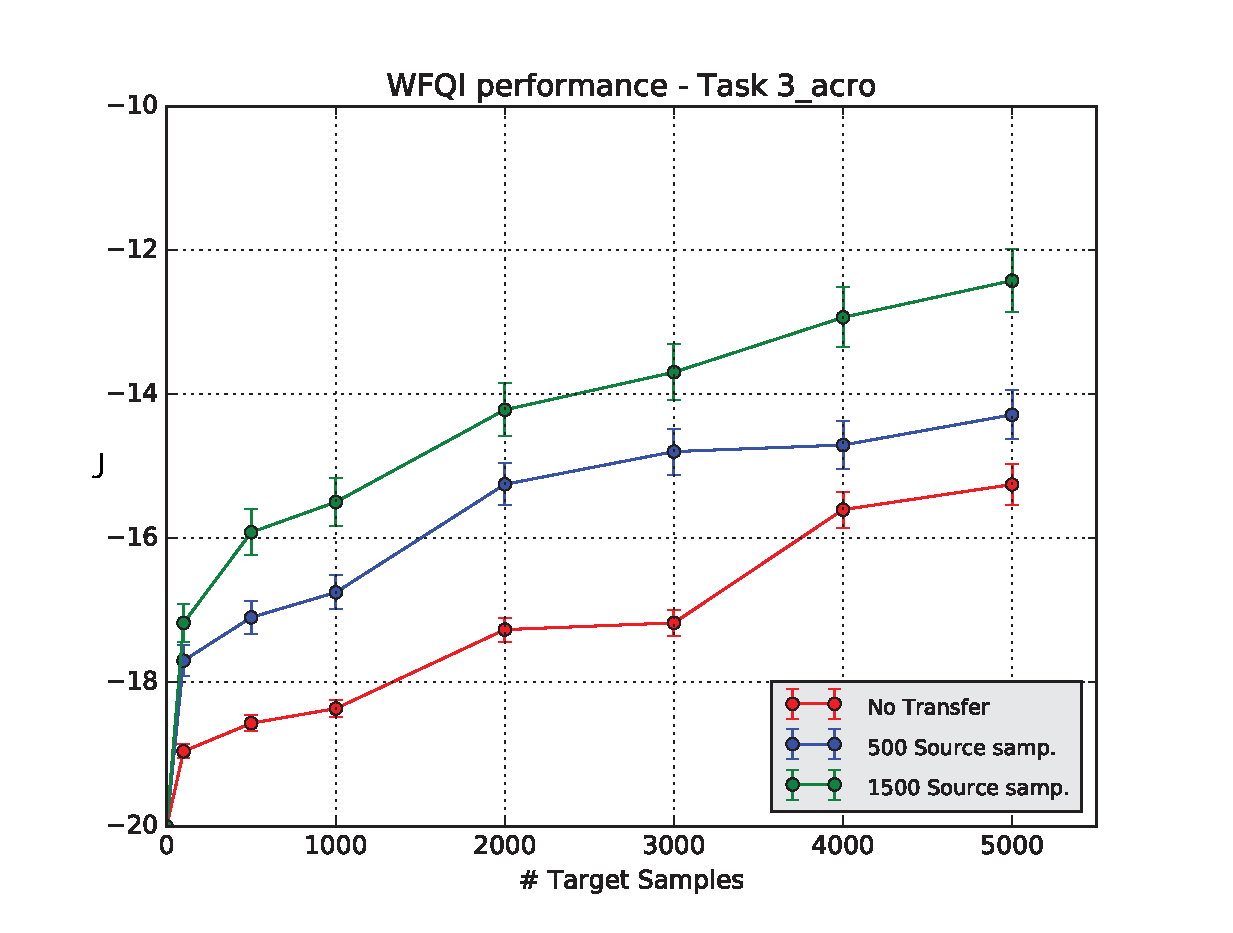
\includegraphics[scale=0.5]{images/WFQIPerf3_acro.eps}
      \caption{WFQI performance Source 3/Target task, est. weights}
      \label{acro3}
    \end{figure}
    %

    \noindent Note that in Source task 2 the performance are lower given that it is very different from the
    target task.\newline
    In the last set of experiments we transfer from all the three source tasks to the target. Again our algorithm
    reveals to be robust toward the effect of the negative transfer (ie. samples from source task 2) and maintains
    an optimal performance using the information coming from the other two.

    \begin{figure}[H]
      \raggedbottom
      \centering
      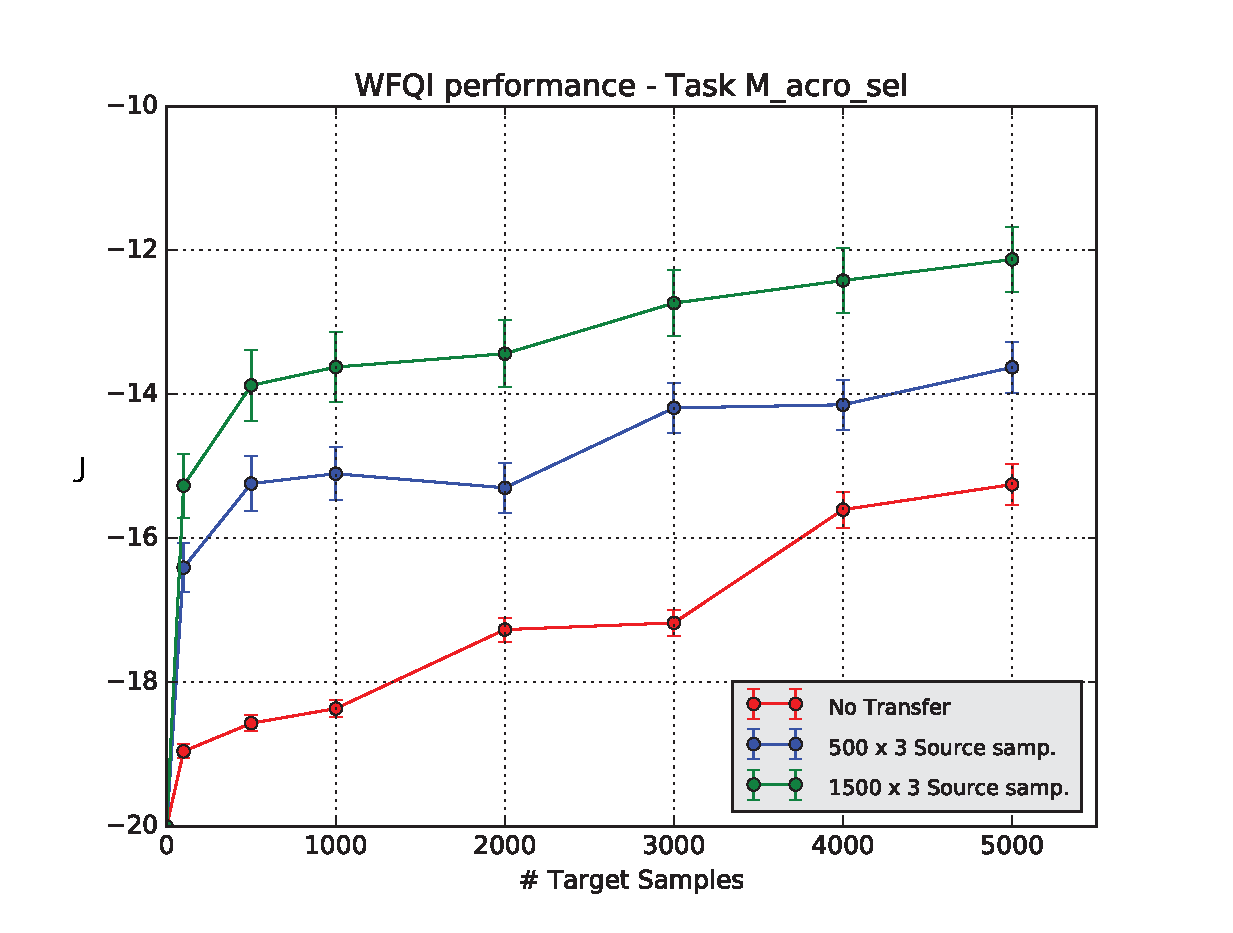
\includegraphics[scale=0.5]{images/WFQIPerfM_acro.eps}
      \caption{WFQI performance Source 1/2/3/Target task, est. weights}
      \label{acro3}
    \end{figure}

    \noindent In addition we also report the results when weights are estimated according to
    Formula \ref{mean-weight} using respectively, in Figure \ref{acro-mean-res1}
    $\sigma^{2}_{p} = 0.09$ and in Figure \ref{acro-mean-res2} $\sigma^{2}_{p} = 0.81$.

    \begin{figure}[H]
      \centering
      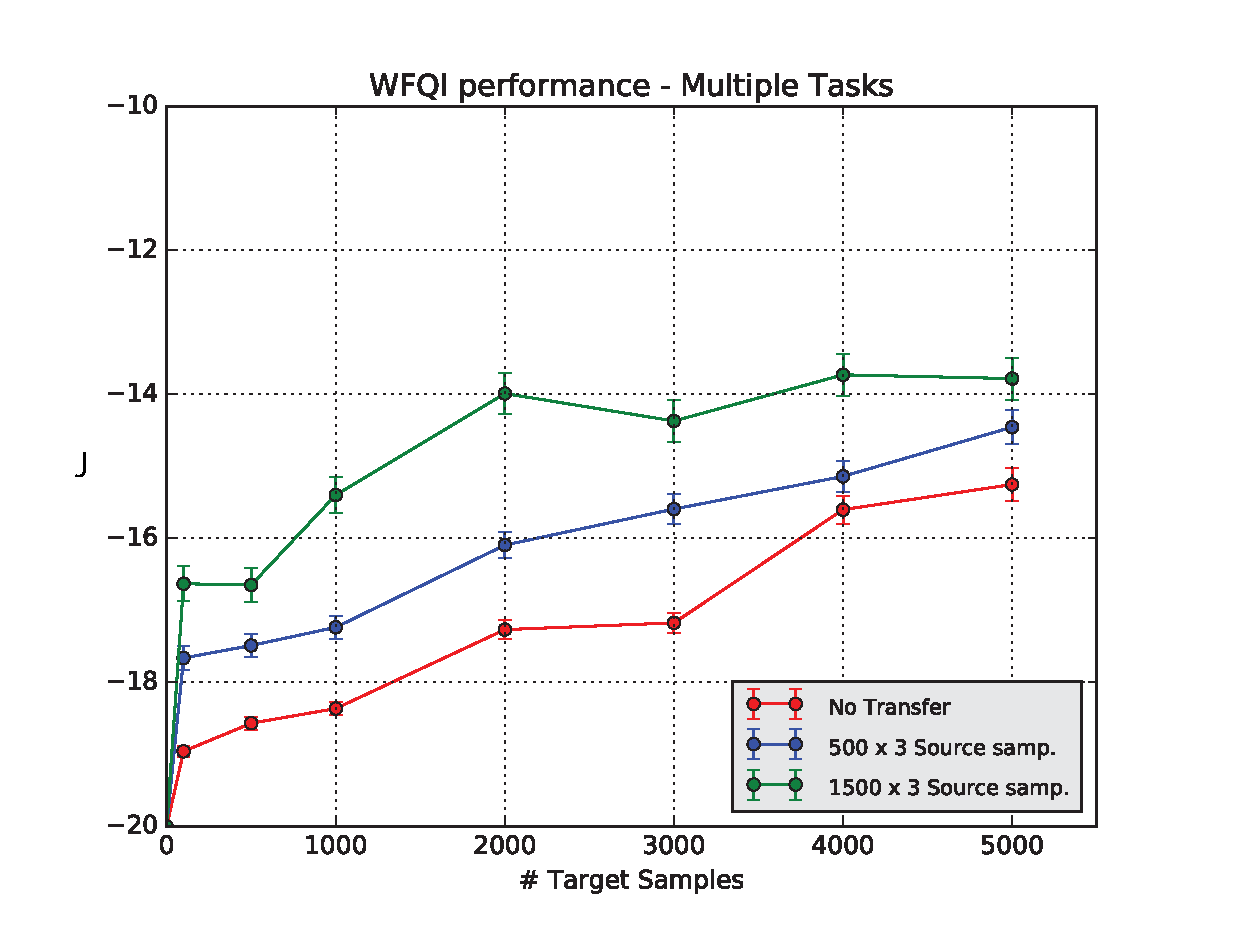
\includegraphics[scale=0.5]{images/WFQIPerfM_acro_MEAN.eps}
      \caption{Acrobot performance, multiple source tasks, Equation \ref{mean-weight} \textbf{without} $\sigma^{2}$ overestimation}
      \label{acro-mean-res1}
    \end{figure}

    \begin{figure}[H]
      \centering
      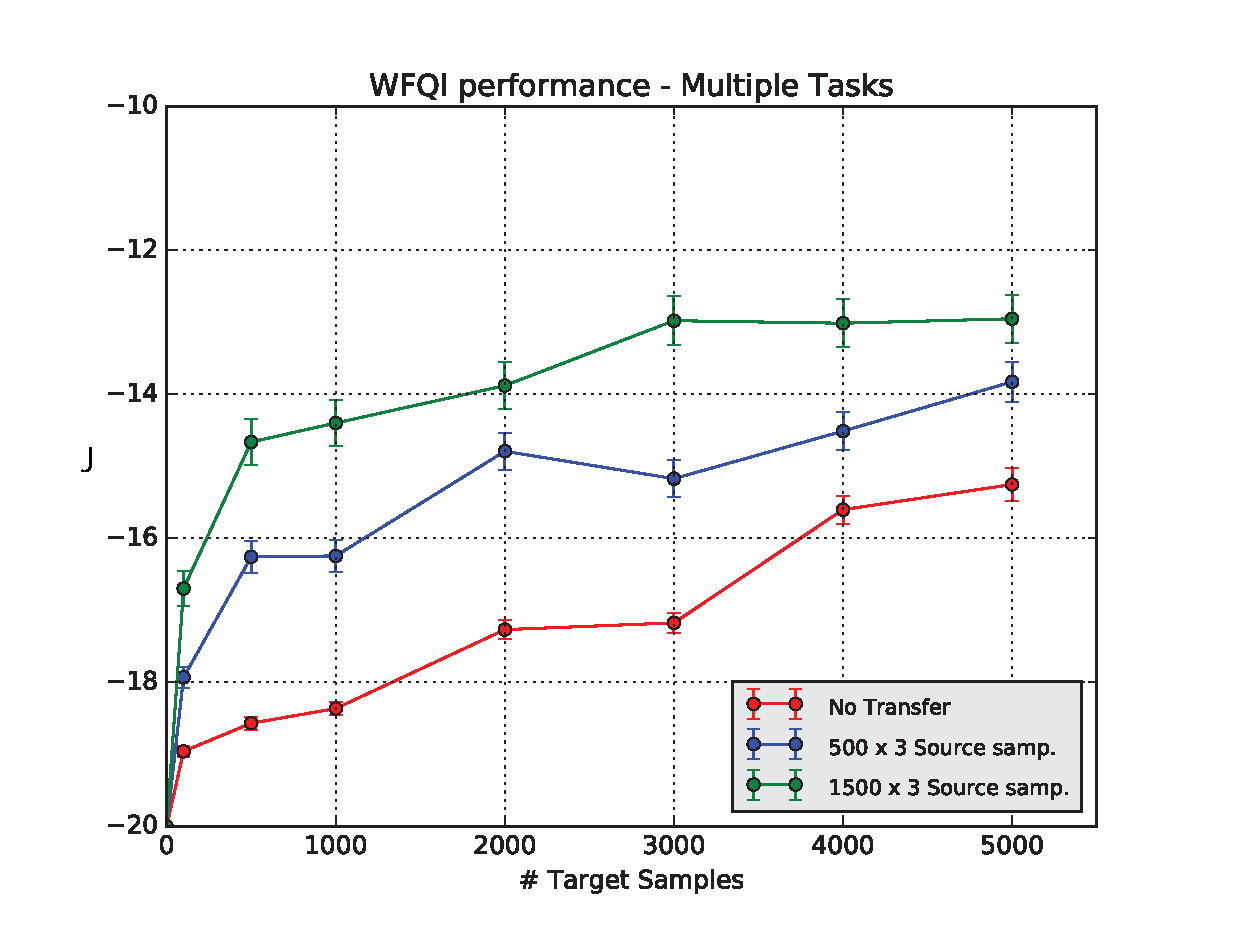
\includegraphics[scale=0.5]{images/WFQIPerfM_acro_MEAN2.eps}
      \caption{Acrobot performance, multiple source tasks, Equation \ref{mean-weight} \textbf{with} $\sigma^{2}$ overestimation}
      \label{acro-mean-res2}
    \end{figure}

    \noindent We observe, in the first case, poor performances, mainly due high number of discarded samples.
    In the second graph we notice a much better performance due to the overestimation of $\sigma^{2}$ for
    both reward and transition model. However notice, in this case, that the performance is not as good as
    in Figure \ref{acro3}. This is mainly due to the fact that Acrobot is a non-gaussian environment
    and $\sigma^{2}$ is just the result of an educated guess and may be not the best choice for this specific
    scenario. Better results could be obtained by using some estimation procedures for $\sigma^{2}$.

  \section{Comparison}
    \noindent In this section we compare our approach with the one presented in \cite{lazaric2008transfer} (abbreviated as BATCH). This
    last approach is based on the calculation of measures between tasks and samples. When the target and source
    tasks share some similarities (in this case the authors assume the tasks to be drawn from the same probability
    distribution $\Omega$) it is possible to measure the distance (called task compliance) between a target and
    a source task, moreover within each source we can measure the likelihood of each sample (sample relevance) to be generated
    in the target task. The algorithm first calculate for each source task the compliance and then for each sample of
    each source, it calculates the relevance. Samples are drawn from each task proportionally to the calculated compliance
    and relevance. For more detail we remand to \cite{lazaric2008transfer}.\newline

    \noindent We compare the performance of WFQI and BATCH over the two environments defined before (Puddle-World and Acrobot).\newline
    For Puddle-World, we use a total of 1000 source samples extracted from the three source tasks at hand. For WFQI the parameters
    are identical to the ones presented in the previous section. For BATCH we maintain the same parameters reported in \cite{lazaric2008transfer}.
    For WFQI calculate weights using the overestimation of $\sigma^{2}$ (in particular we take $\sigma^{2} = 0.09$).

    \begin{figure}[H]
      \centering
      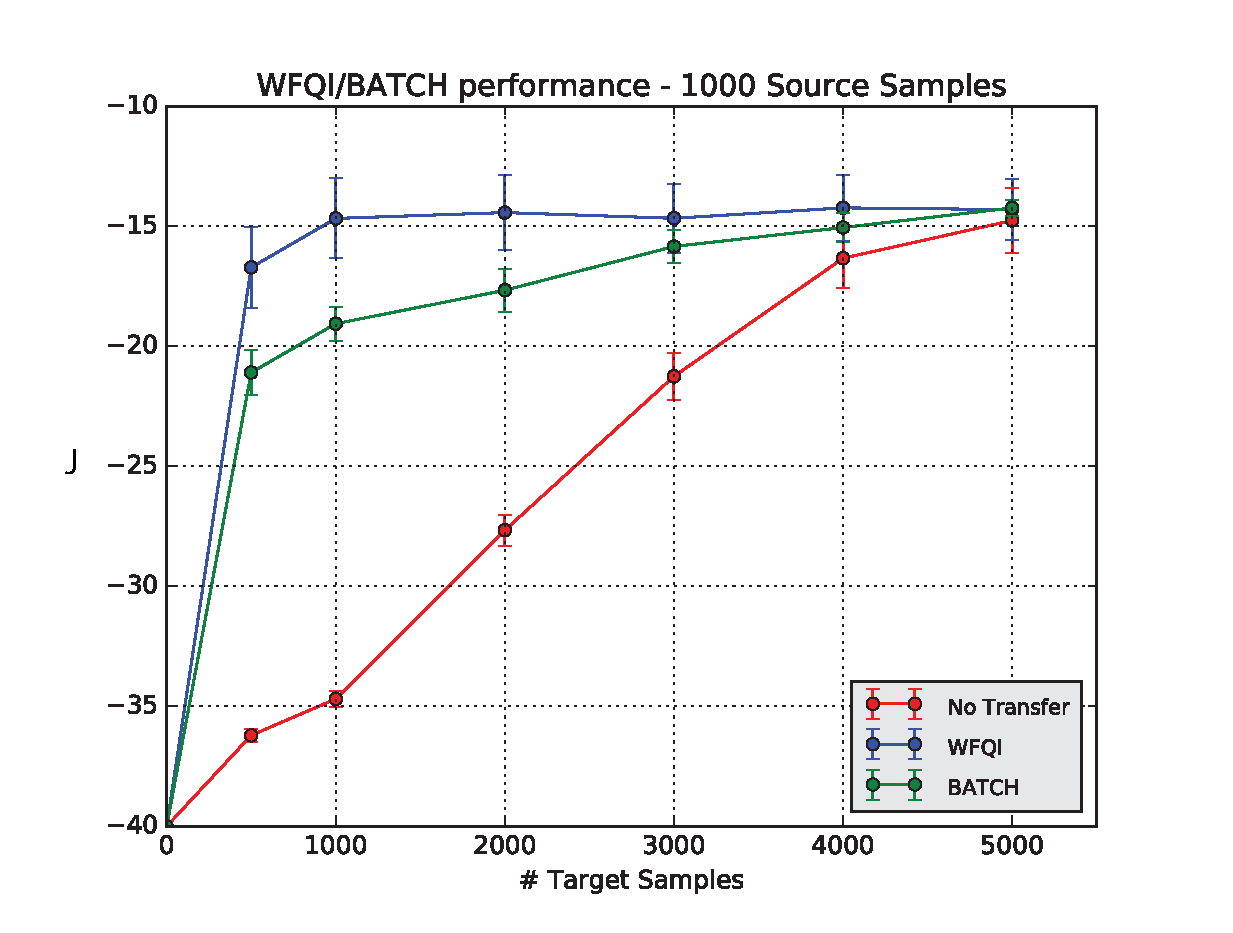
\includegraphics[scale=0.5]{images/WFQIPerfCMP.eps}
      \caption{Puddle World - Performance comparison BATCH vs WFQI}
      \label{}
    \end{figure}


    \noindent Notice how our approach is able to gain a better jumpstart performance over BATCH when the number of target samples is low.\newline

    \noindent Moreover we propose a similar comparison also over the Acrobot environment. In this case 1000 source samples are used,
    parameters for WFQI are unchanged with respect to the previous case. For BATCH we use ($\delta_{s,a}=0.3, \delta_{r}=0.5, \delta_{p}=0.3, \mu=0.5$) all
    the other parameters regarding FQI are unchanged with respect the ones presented in the previous set of experiments.
    \begin{figure}[H]
      \centering
      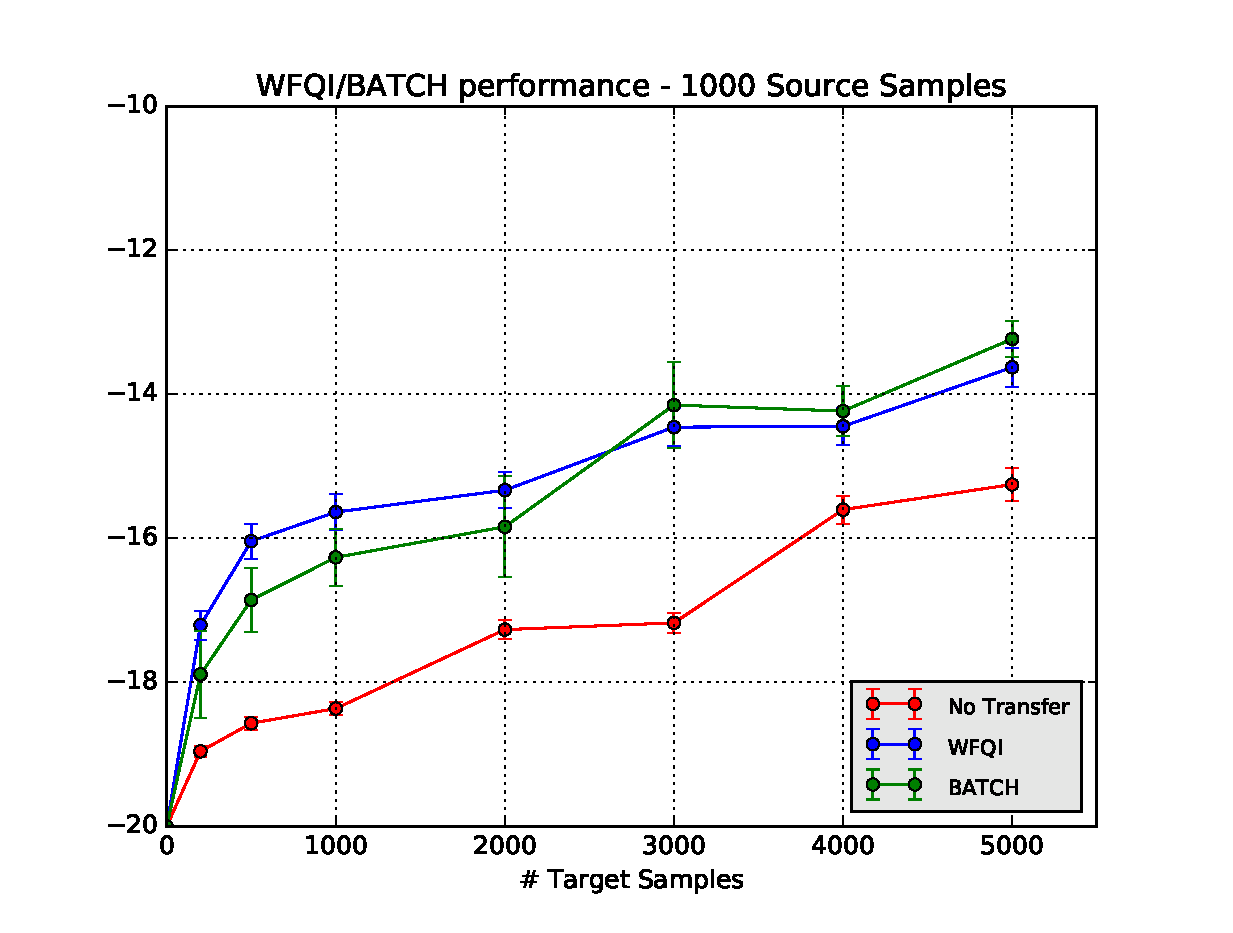
\includegraphics[scale=0.5]{images/WFQIPerfCMPacro.eps}
      \caption{Acrobot - Performance comparison BATCH vs WFQI}
      \label{}
    \end{figure}
    \noindent Again we notice how WFQI is able to gain an advantage in the first part of the test, when the number of
    target samples is low, but in the final part the performance are identical.


    %
